\documentclass{beamer}

\usetheme{metropolis} % Usa Metropolis
\usepackage{graphicx}
\usepackage{booktabs}
\usepackage{amsmath}
\usepackage{siunitx}
% \usepackage[sort&compress,numbers]{natbib} % Citas bibliográficas
\usepackage[style=authoryear,backend=biber]{biblatex}
\usepackage{hyperref}
\usepackage[utf8]{inputenc}
\usepackage{fontspec}
\usepackage{textalpha}

\addbibresource{../Bibliography/Thesis_unified.bib}

% Logo en la esquina inferior derecha (ajusta el path si tienes un logo)
\setbeamertemplate{footline}{
  \leavevmode%
  \vspace{0.3cm}
  \hbox{%
  \hspace*{0.5cm}
  
\includegraphics[height=0.5cm]{images_link/Cinvestav-logo.png}\hspace*{0.5cm}%
  \insertframenumber{} de \inserttotalframenumber\hspace*{0.5cm}
  }%
}

% Acrónimos (opcional)
% \usepackage[acronym]{glossaries}
% \makeglossaries
% \newacronym{qcd}{QCD}{Quantum Chromodynamics}

\graphicspath{{figures/}{images_link/}}

\title{Distribución de presión dentro de nucleones en un modelo de bolsa Tsallis-MIT}
\subtitle{Defensa de Tesis Doctoral}
\author{Manuel Alejandro Matías Astorga}
\date{
  \vspace{0.5em}
  Asesor: Dr. Gerardo Herrera Corral\\
  \today \hfill 
\includegraphics[width=0.2\linewidth]{images_link/Cinvestav-logo.png}
}
\institute{CINVESTAV IPN}
%----------------------------------------------------------------------------------%
\begin{document}

\maketitle

\begin{frame}{Contenido}
  \tableofcontents
\end{frame}

\section[Introducción]{1. Introducción}
% \begin{frame}{¿Qué es un protón?}
%   \begin{itemize}
%     \item Partícula compuesta: quarks y gluones\cite{Barboza_Mendoza_2019}
%     \item Confinamiento: propiedad fundamental de la QCD
%     \item ¿Cómo explorar su estructura interna?
%   \end{itemize}
% \end{frame}

\begin{frame}{Confinamiento e Interacción Fuerte}
  \begin{columns}
    % Columna izquierda: contenido animado
    \column{0.55\textwidth}
  
    % Paso 1: Confinamiento
    \only<1>{
      \begin{itemize}
        \item[] \textbf{Los quarks no existen libres en la naturaleza.}
        \item[] Se encuentran siempre confinados dentro de hadrones (bariones, mesones).
        \item[] La separación genera energía que produce nuevos pares \( q\bar{q} \).
      \end{itemize}
    }
  
    % Paso 2: Potencial Huang
    \only<2>{
      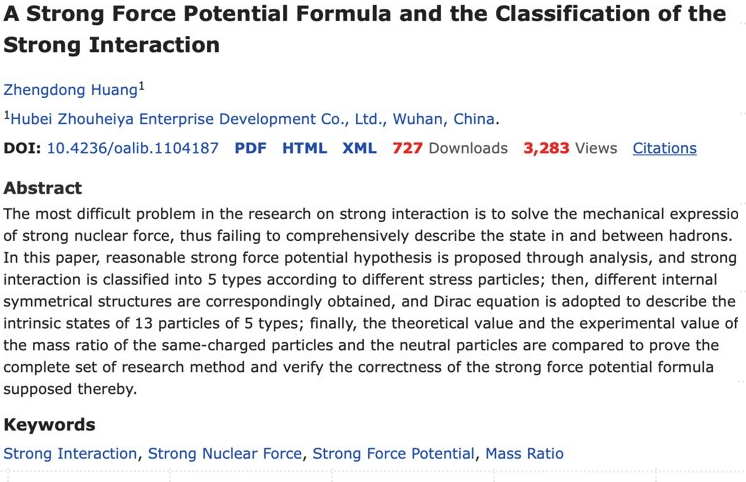
\includegraphics[width=0.9\linewidth]{figures/potencial_fuerza.png}
      \vspace{0.5em}
      \begin{equation*}
      V(r) = \frac{-3\hbar c}{2r} e^{\pm 2(r/a - 1)}
      \end{equation*}
      \scriptsize Fuente: \cite{huangStrongForcePotential2018}
    }
  
    % Paso 3: Potencial lineal aproximado
    \only<3>{
      \begin{equation*}
      V(r) \approx -\frac{k_1}{r} + k_2 r
      \end{equation*}
      \begin{itemize}
        \item Término \(-k_1/r\): atracción tipo Coulomb.
        \item Término \(k_2 r\): confinamiento a largas distancias.
      \end{itemize}
    }
  
    % Columna derecha: imagen fija
    \column{0.45\textwidth}
    \centering
    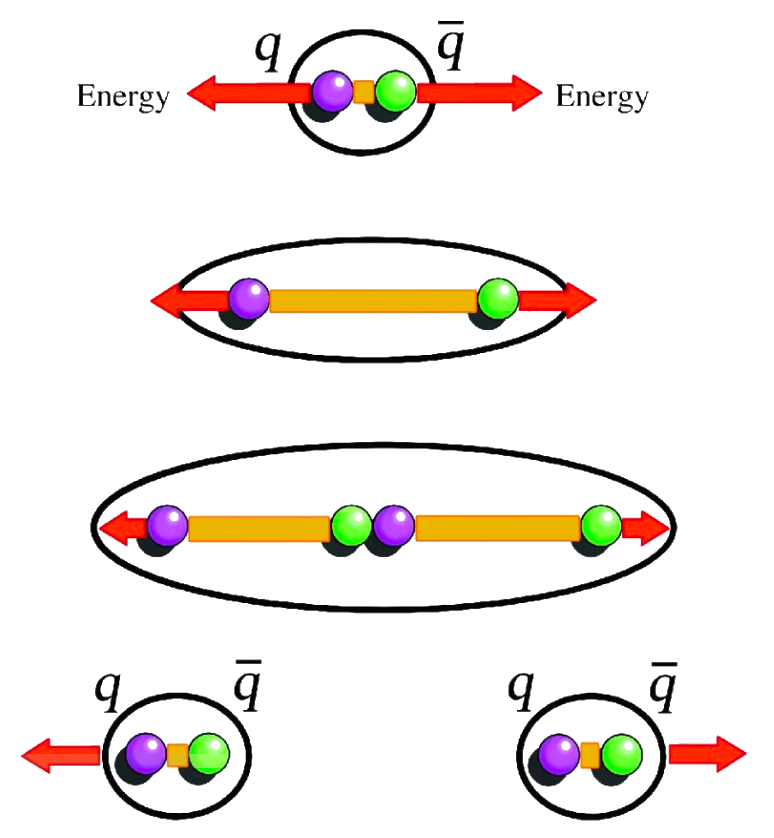
\includegraphics[width=\linewidth]{figures/confinamiento.png}
  
  \end{columns}
  \end{frame}

\begin{frame}{Interpretación física}
\begin{equation*}
V(r) \approx -\frac{k_1}{r} + k_2 r
\end{equation*}
\begin{itemize}
  \item \(k_2\) refleja la tensión del "tubo de flujo" de gluones.
  \item A escala de \(r \sim 1\) fm: \(k_2 \sim 1\,\mathrm{GeV/fm}\).
  \item Quarks no pueden escapar: ¡el confinamiento es inevitable!
\end{itemize}
\end{frame}

\begin{frame}{Constante de acoplamiento fuerte}
\begin{equation*}
\alpha_s(E) = \frac{12\pi}{(33 - 2n_f)\ln\left(\frac{E^2}{\Lambda^2}\right)}
\end{equation*}
\begin{itemize}
  \item A escalas bajas \( E \sim \SI{1}{GeV} \): \( \alpha_s \sim 1 \) → confinamiento fuerte.
  \item A altas energías: \( \alpha_s \ll 1 \) → libertad asintótica.
  \item Quarks se comportan como libres cuando están muy cerca.
\end{itemize}
\end{frame}

\begin{frame}[standout]
  \Large\textbf{¡Libertad Asintótica!}
  \\[1em]
  La interacción fuerte se debilita a altas energías → los quarks se "liberan" temporalmente.
\end{frame}
%%%%%%%%%%%%%%%%%%%%%%%%%%%%%%%%%%%%%%%%%%%%%%%%%%%%%%%%%%%%%%%%%%%%%%%%%%%%%%%%%%%%%
\begin{frame}{Jets de mesones: evidencia de confinamiento}
  \begin{columns}
    \column{0.55\textwidth}
    \only<1>{
      \begin{itemize}
        \item Colisión \( pp \) a \( \sqrt{s} = 13\,\mathrm{TeV} \)
        \item Producción de quarks a altas energías
      \end{itemize}
    }
    \only<2>{
      \begin{itemize}
        \item En el laboratorio no se detectan quarks libres
        \item Se observan \textbf{jets} de partículas neutras (mesones, bariones)
      \end{itemize}
    }
    \only<3>{
      \begin{itemize}
        \item Este fenómeno se conoce como \textbf{hadronización}
        \item Proceso guiado por la interacción fuerte
      \end{itemize}
    }
    \only<4>{
      \begin{itemize}
        \item Se describe formalmente con diagramas de Feynman
        \item Evalúa amplitudes de probabilidad para procesos de colisión
      \end{itemize}
    }
    \only<5>{
      \begin{itemize}
        \item Producción de hadrones aumenta cuando se alcanza el umbral de energía
        \item Aparece un nuevo sabor de quark disponible
      \end{itemize}
    }

    \column{0.45\textwidth}
    \centering
    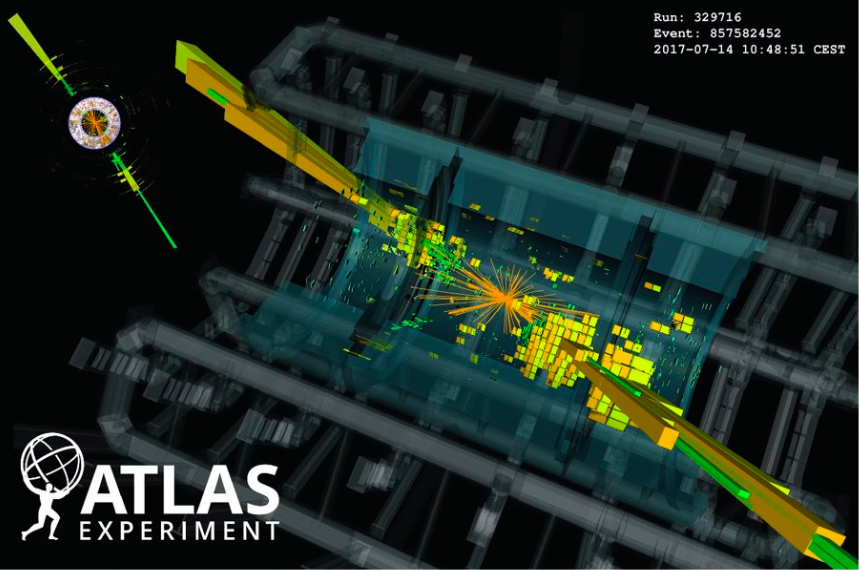
\includegraphics[width=\linewidth]{figures/atlas_detector.png}
  \end{columns}
\end{frame}

\begin{frame}{Jets de mesones: del modelo al experimento}
  \begin{columns}
    \column{0.55\textwidth}
    \small
    \begin{itemize}
      \item Diagrama de Feynman: producción de \(\mu^+\mu^-\) y \(q\bar{q}\).
      \item A mayor energía de colisión, se abren canales para nuevos sabores de quarks.
      \item Cada nuevo sabor disponible incrementa la producción de hadrones.
      \item Esto se refleja en la fórmula de secciones eficaces:
    \end{itemize}
    \vspace{0.5em}
    \[
    \sigma_{e^+e^- \to \mu^+\mu^-} = \sigma_0 \quad \quad
    \sigma_{e^+e^- \to q\bar{q}} = \left( \sum_f q_f^2 \right)\sigma_0
    \]
    \column{0.45\textwidth}
    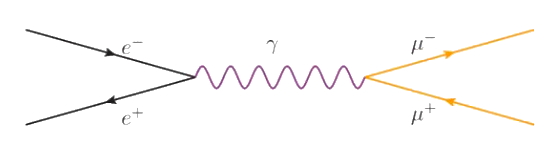
\includegraphics[width=\linewidth]{figures/feynman_diagrams1-2.png}
    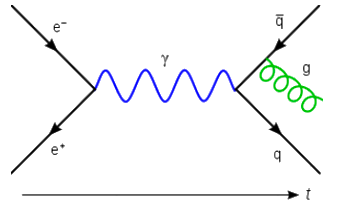
\includegraphics[width=\linewidth]{figures/feynman_diagrams2-2.png}
  \end{columns}
\end{frame}

\begin{frame}{Razón de producción de pares}
  \begin{columns}
    \column{0.5\textwidth}
    \[
    R = \frac{\sigma_{e^+e^- \to q\bar{q}}}{\sigma_{e^+e^- \to \mu^+\mu^-}} = \left( \sum_f q_f^2 \right)
    \]
    \begin{itemize}
      \item Relación entre secciones eficaces permite identificar la aparición de nuevos sabores.
      \item El gráfico muestra resonancias hadrónicas conforme aumenta \(\sqrt{s}\).
      \item Cada pico indica la activación de un nuevo canal de producción.
    \end{itemize}
    \column{0.5\textwidth}
    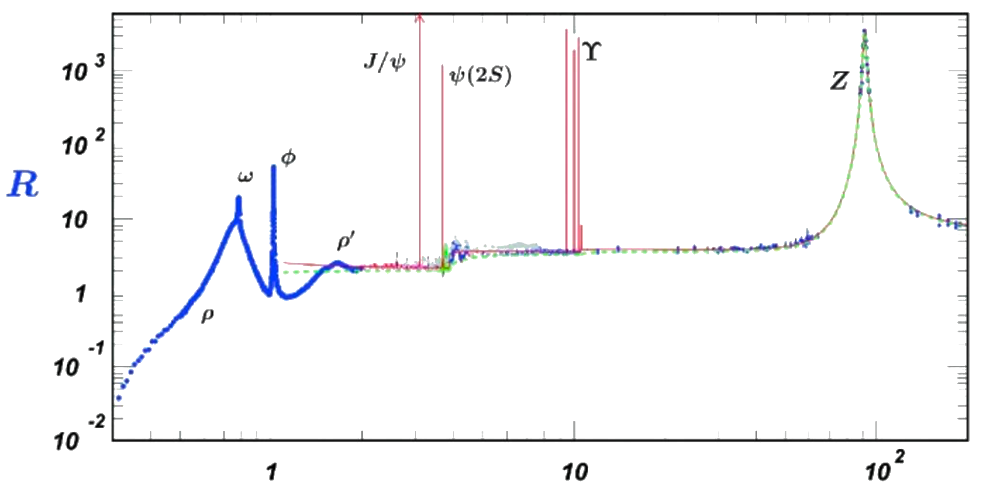
\includegraphics[width=\linewidth]{figures/produccion_pares.png}
  \end{columns}
  \vspace{0.5em}
  \centering
  {\scriptsize Energía de centro de masa \(\sqrt{s}\) en GeV}
\end{frame}

\begin{frame}{Cromodinámica cuántica (QCD)}
  \begin{columns}
    \column{0.55\textwidth}
    \begin{equation*}
      \langle q_b | e^{-iH(t_b - t_a)/\hbar} | q_a \rangle = \int \mathcal{D}(q) e^{i S(q)/\hbar}
    \end{equation*}
    \begin{equation*}
      S(q) = \int_{t_a}^{t_b} \mathcal{L}(q, \dot{q})\,dt
    \end{equation*}
    \vspace{1em}
    \begin{equation*}
      \mathcal{L}_{\text{QCD}} = -\frac{1}{4} F_{\mu\nu}^a F^{\mu\nu}_a + \sum_{q=u,d,s,...} \bar{q}(\gamma^\mu D_\mu + m_q)q
    \end{equation*}

    \column{0.45\textwidth}
    \centering
    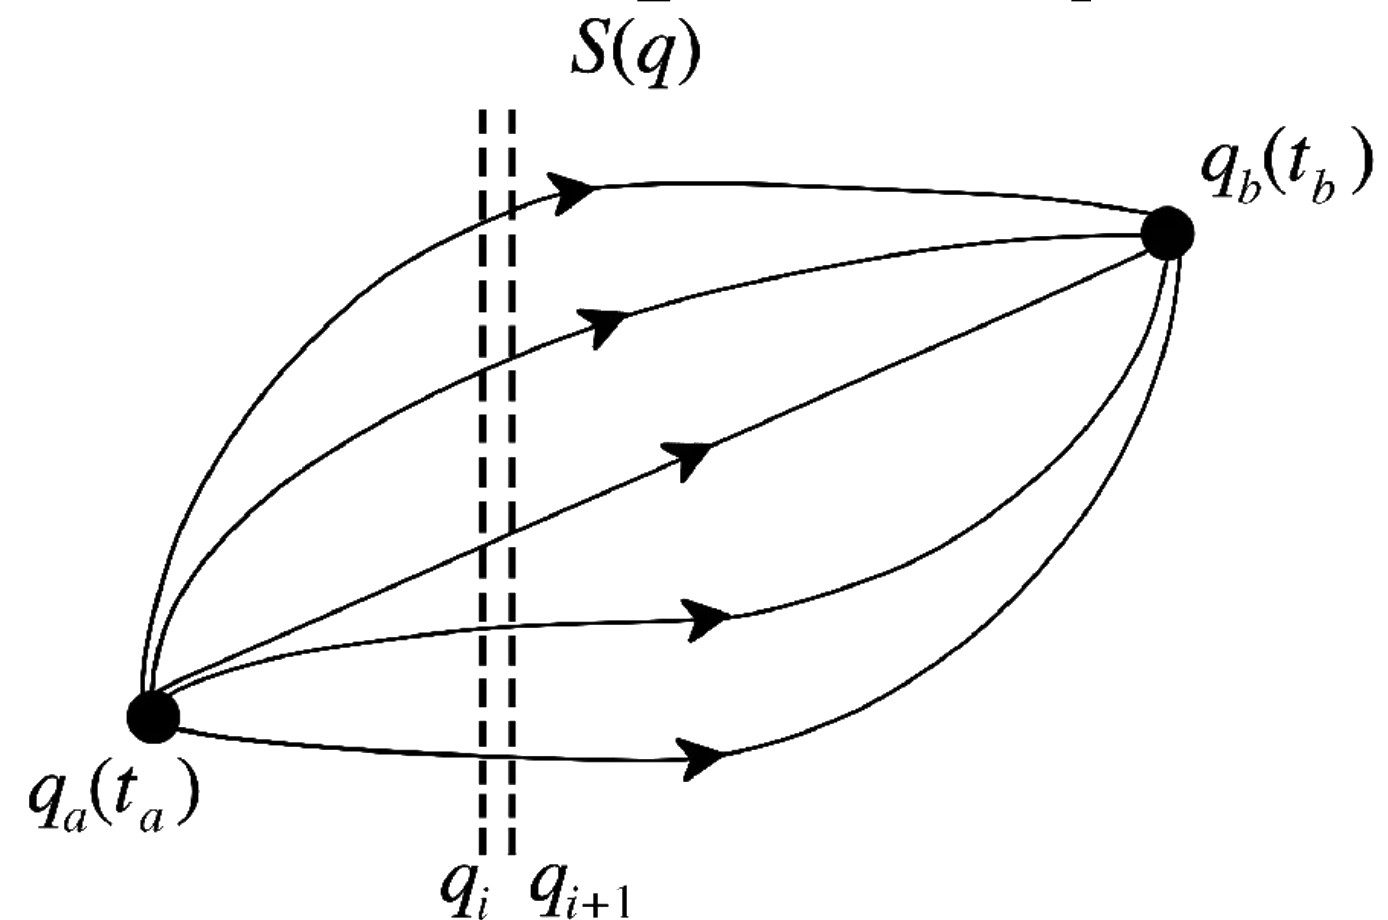
\includegraphics[width=\linewidth]{figures/qcd_path_integral.png}
  \end{columns}
\end{frame}

\begin{frame}{Lattice QCD}
  \begin{columns}
    \column{0.55\textwidth}
    \begin{itemize}
      \item El campo de quarks se representa en nodos discretos.
      \item El campo de gluones en los enlaces entre nodos (matrices \( U_\mu(x) \)).
      \item Las integrales funcionales se discretizan como productos.
      \item Se requiere simulación Monte Carlo.
    \end{itemize}
    \vspace{1em}
    \begin{equation*}
      \int D\psi D\bar{\psi} DA \to \prod_{n} d\psi(an) d\bar{\psi}(an) dU(an)
    \end{equation*}
    \begin{equation*}
      U_\mu(x) = \exp(iga A_\mu(x + \hat{\mu}/2))
    \end{equation*}

    \column{0.45\textwidth}
    \centering
    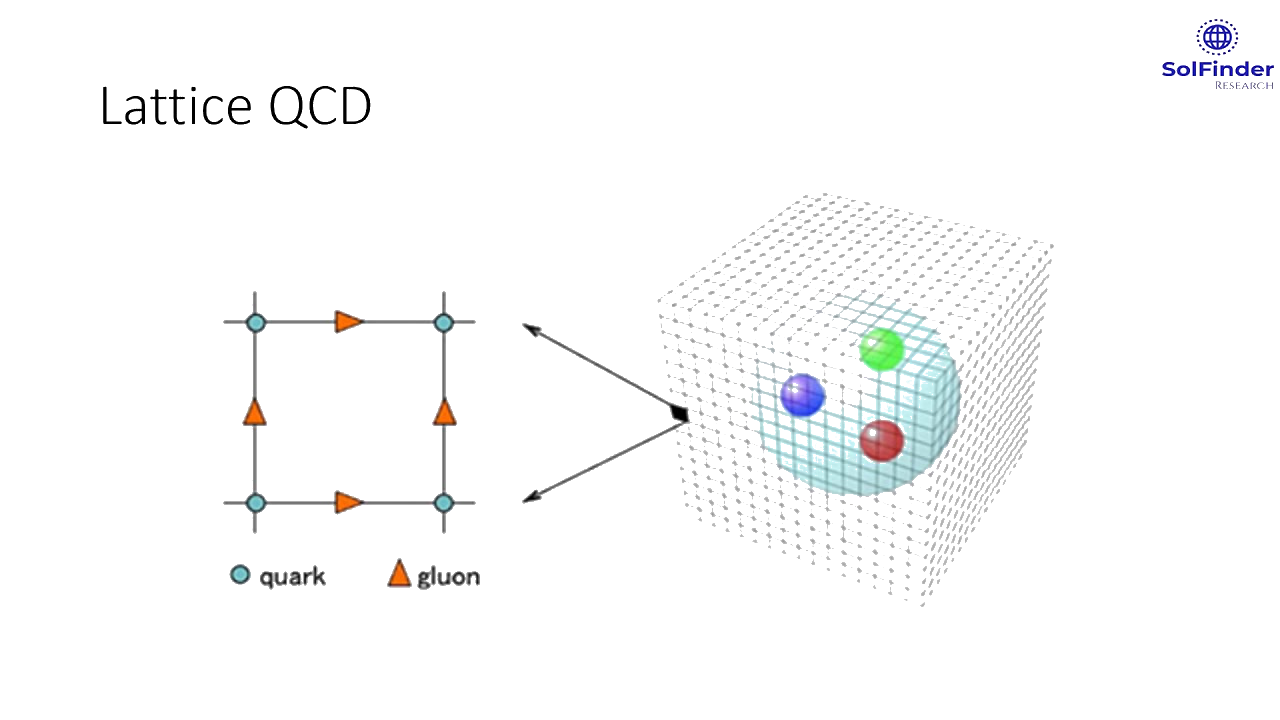
\includegraphics[width=\linewidth]{figures/lattice_qcd.png}
  \end{columns}
\end{frame}

  

\begin{frame}{Resultados de LQCD: correlaciones nucleares}
  \begin{columns}
    \column{0.33\textwidth}
    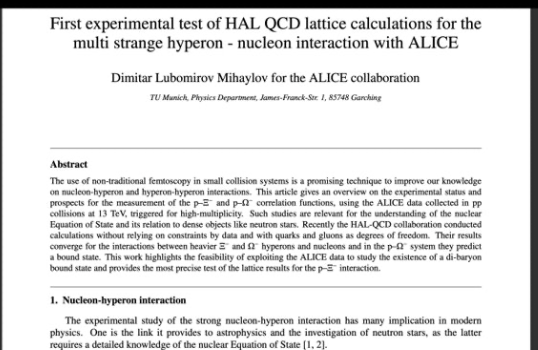
\includegraphics[width=\linewidth]{figures/alice_hal_qcd_paper.png}
    \column{0.33\textwidth}
    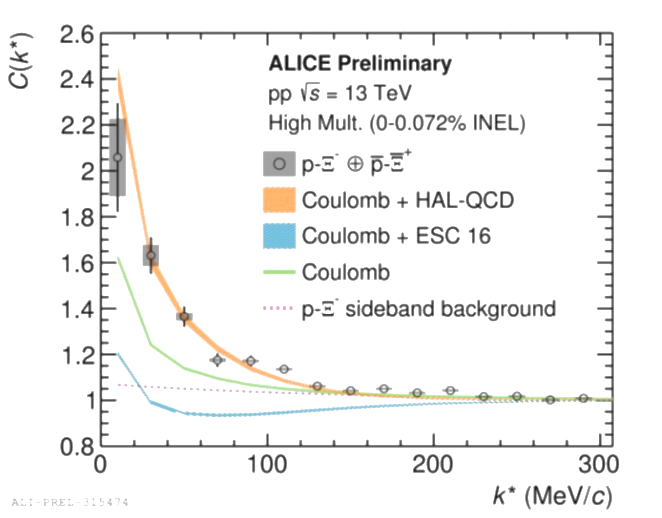
\includegraphics[width=\linewidth]{figures/alice_corr1.png}
    \column{0.33\textwidth}
    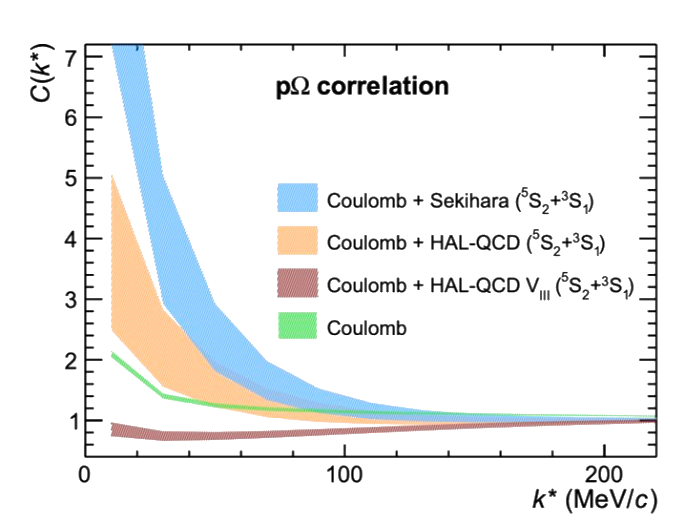
\includegraphics[width=\linewidth]{figures/alice_corr2.png}
  \end{columns}
  \vspace{1em}
  \scriptsize Cálculos de HAL-QCD validados con datos experimentales de ALICE (\( pp \) a 13 TeV).
\end{frame}

\begin{frame}{Distribución de presión dentro del protón}
  \begin{columns}
    \column{0.4\textwidth}
    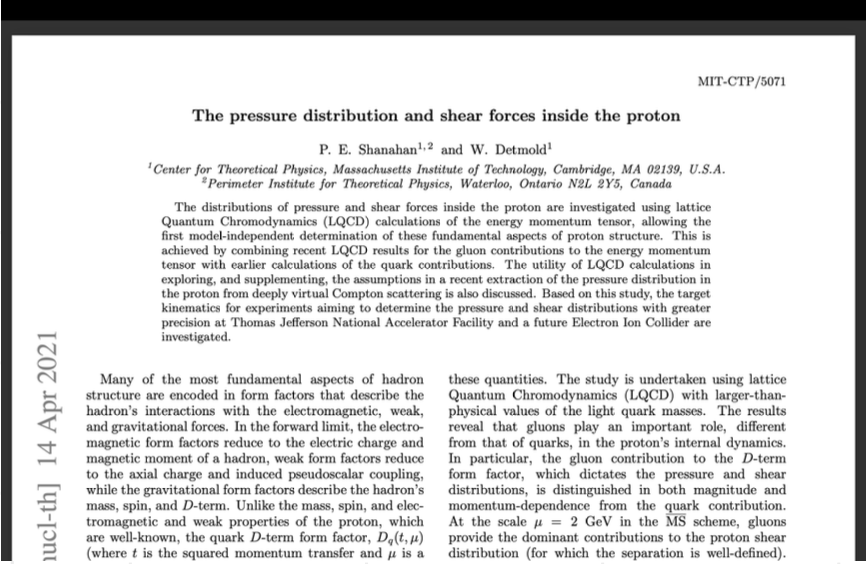
\includegraphics[width=\linewidth]{figures/shanahan_pressure_paper.png}
    \column{0.6\textwidth}
    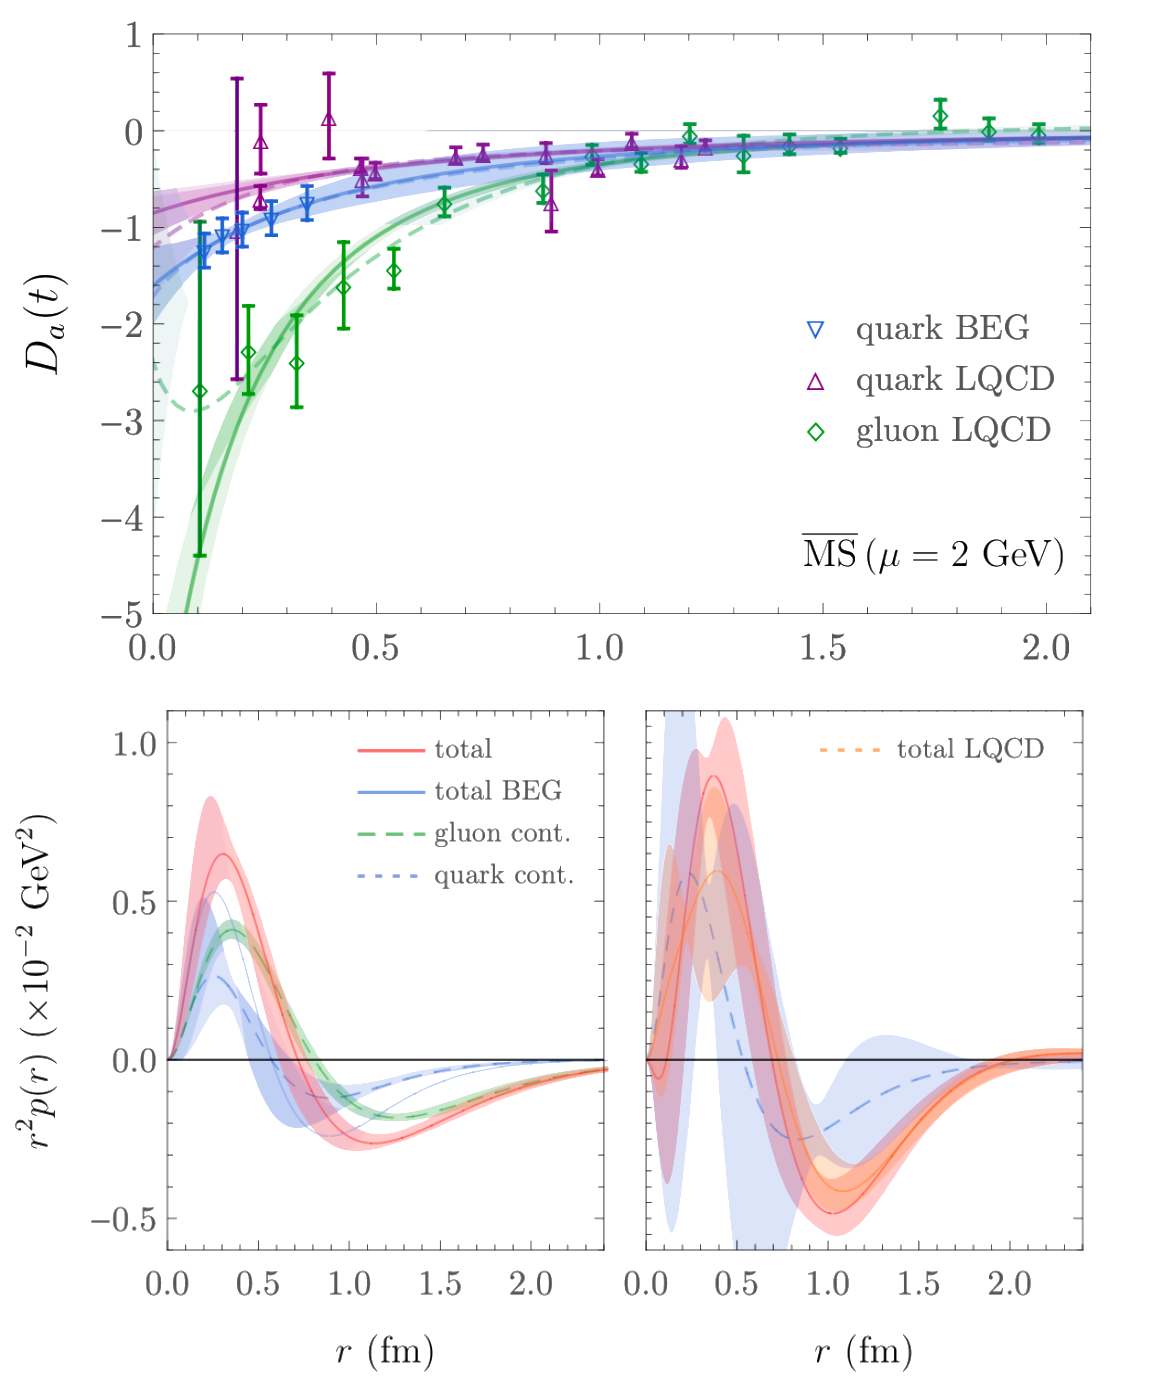
\includegraphics[width=0.8\linewidth]{figures/shanahan_pressure_plots.png}
  \end{columns}
  \vspace{1em}
  \scriptsize Resultados de LQCD + parametrizaciones (BEG) para la distribución de presión y función \( D \).
\end{frame}

\begin{frame}[standout]
  \Large\textbf{Limitaciones de LQCD}
  \vspace{1em}

  \begin{enumerate}[i.]
    \item Método Monte Carlo no funciona con interacciones repulsivas.
    \item Problema del signo impide resolver ciertas integrales en tiempo real.
    \item Limita los escenarios accesibles en QCD a partir de LQCD.
  \end{enumerate}
\end{frame}


%%%%%%%%%%%%%%%%%%%%%%%%%%%%%%%%%%%%%%%%%%%%%%%%%%%%%%%%%%%%%%%%%%%%%%%%%%%%%%%%%%%%%

\section[Modelo de Bolsa del MIT]{2. Modelo de Bolsa del MIT}
\begin{frame}{El modelo de bolsa del MIT}
  \begin{columns}
    % Columna izquierda: ecuaciones animadas
    \column{0.55\textwidth}

    \only<1>{
      \begin{block}{Ecuación de Dirac sin masa}
      \begin{equation*}
        (i \gamma^\mu \partial_\mu - m) \psi = 0, \quad m = 0
      \end{equation*}
      \end{block}
      \vspace{-1.5em}
      \begin{equation*}
        i\partial_\mu = (p^0, \mathbf{p})
      \end{equation*}
      \begin{equation*}
        \gamma^0 = \begin{pmatrix}
        \mathbb{I} & 0\\
        0 & -\mathbb{I}
        \end{pmatrix}, \quad
        \gamma^i = \begin{pmatrix}
        0 & \sigma^i\\
        -\sigma^i & 0
        \end{pmatrix}
      \end{equation*}
    }

    \only<2>{
      \begin{block}{Representación de espinores}
      \begin{equation*}
        \psi = \begin{pmatrix}
        \psi_+\\
        \psi_-
        \end{pmatrix}
      \end{equation*}
      \end{block}
    }

    \only<3>{
      \begin{block}{Forma matricial de Dirac}
      \begin{equation*}
        \begin{pmatrix}
        p^0 & -\boldsymbol{\sigma}\cdot\mathbf{p} \\
        \boldsymbol{\sigma}\cdot\mathbf{p} & -p^0
        \end{pmatrix}
        \begin{pmatrix}
        \psi_+\\
        \psi_-
        \end{pmatrix} = 0
      \end{equation*}
      \end{block}
      \vspace{-1.2em}
      \begin{align*}
        \psi_+(\mathbf{r}, t) &= \mathcal{N} e^{-i p^0 t} j_0(p^0 r) \chi_+\\
        \psi_-(\mathbf{r}, t) &= \mathcal{N} e^{-i p^0 t} \boldsymbol{\sigma} \cdot \hat{r} j_1(p^0 r) \chi_-
      \end{align*}
    }

    \only<4>{
      \begin{block}{Condición de frontera}
      \begin{align*}
        \bar{\psi} \psi \big|_{r=R} &= [j_0(p^0 R)]^2 - \boldsymbol{\sigma} \cdot \hat{r} \, [j_1(p^0 R)]^2 = 0
      \end{align*}
      \end{block}
      \vspace{-1em}
      \begin{equation*}
        \Rightarrow \quad p^0_m = \frac{2.04}{R}
      \end{equation*}
    }

    % Columna derecha: imagen fija
    \column{0.45\textwidth}
    \centering
    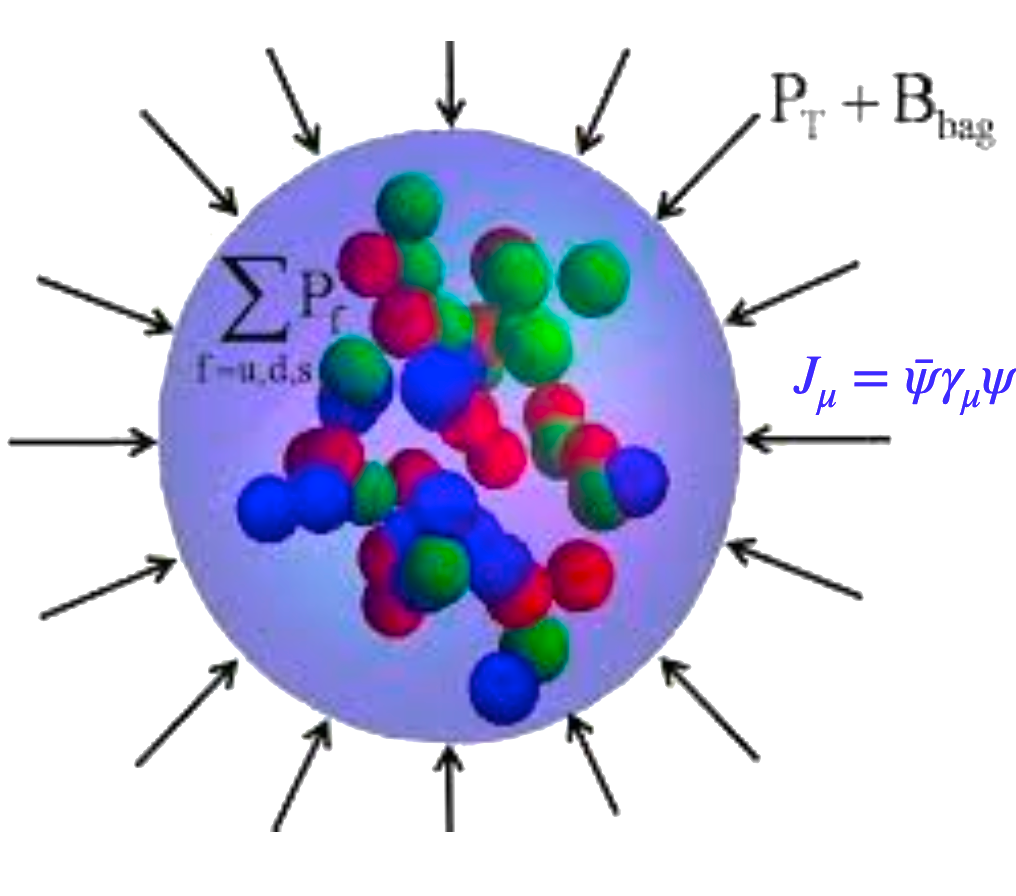
\includegraphics[width=\linewidth]{figures/mit_bag_model.png}
  \end{columns}
\end{frame}

\begin{frame}{La presión total – Gas de Bose-Einstein ultrarrelativista}
  \begin{columns}
    \column{0.65\textwidth}
    
    \only<1>{
      \centering
      \begin{equation*}
        \Xi^{\text{BE}}(T,V,\mu) = \prod_{k=1}^\infty \frac{1}{1 - \xi e^{-\beta \varepsilon_k}},
        \quad
        \beta = \frac{1}{k_B T},
        \quad
        \xi = e^{\beta \mu}
      \end{equation*}
    }

    \only<2>{
      \centering
      \begin{align*}
        \langle n_k \rangle &= -\frac{1}{\beta} \frac{\partial}{\partial \varepsilon_k} \ln \Xi
        \quad\Rightarrow\quad
        \langle n_k \rangle = \frac{1}{\xi^{-1} e^{\beta \varepsilon_k} - 1}
      \end{align*}
    }

    \only<3>{
      \centering
      \begin{align*}
        N(T,V,\mu) &= \sum_k \langle n_k \rangle\\
        E(T,V,\mu) &= \sum_k \langle n_k \rangle \varepsilon_k
      \end{align*}
    }

    \only<4>{
      \centering
      \begin{align*}
        N(T,V,\mu) &= \frac{4\pi V}{(hc)^3} \int_0^\infty \frac{\varepsilon^2 \, d\varepsilon}{\xi^{-1} e^{\beta \varepsilon} - 1}\\
        E(T,V,\mu) &= \frac{4\pi V}{(hc)^3} \int_0^\infty \frac{\varepsilon^3 \, d\varepsilon}{\xi^{-1} e^{\beta \varepsilon} - 1}
      \end{align*}
    }

    \only<5>{
      \centering
      \begin{align*}
        \mu &= 0 \quad \Rightarrow \quad \xi = 1\\[0.5em]
        N(T,V) &= \frac{4\pi V}{(hc)^3} \int_0^\infty \frac{\varepsilon^2 \, d\varepsilon}{e^{\beta \varepsilon} - 1}\\
        E(T,V) &= \frac{4\pi V}{(hc)^3} \int_0^\infty \frac{\varepsilon^3 \, d\varepsilon}{e^{\beta \varepsilon} - 1}
      \end{align*}
    }

    \only<6>{
      \centering
      \begin{align*}
        N(T,V) &= \frac{1}{\pi^2} \zeta(3) VT^3\\
        E(T,V) &= \frac{\pi^2}{30} VT^4
      \end{align*}
    }

    \only<7>{
      \textbf{Para gluones:} \( g_G = 8 \times 2 = 16 \)
      \begin{align*}
        N_G(T,V) &= \frac{g_G}{\pi^2} \zeta(3) VT^3\\
        E_G(T,V) &= g_G \frac{\pi^2}{30} VT^4
      \end{align*}
    }

    \only<8>{
      \begin{align*}
        P &= \frac{4\pi}{(hc)^3} \cdot \frac{1}{3} \int_0^\infty \frac{\varepsilon^3 \, d\varepsilon}{e^{\beta \varepsilon} - 1}
        \Rightarrow \frac{1}{3} \frac{E}{V}
        = \frac{g_G \pi^2}{90} T^4
      \end{align*}
    }

    \column{0.35\textwidth}
    \centering
    \only<7-8>{
      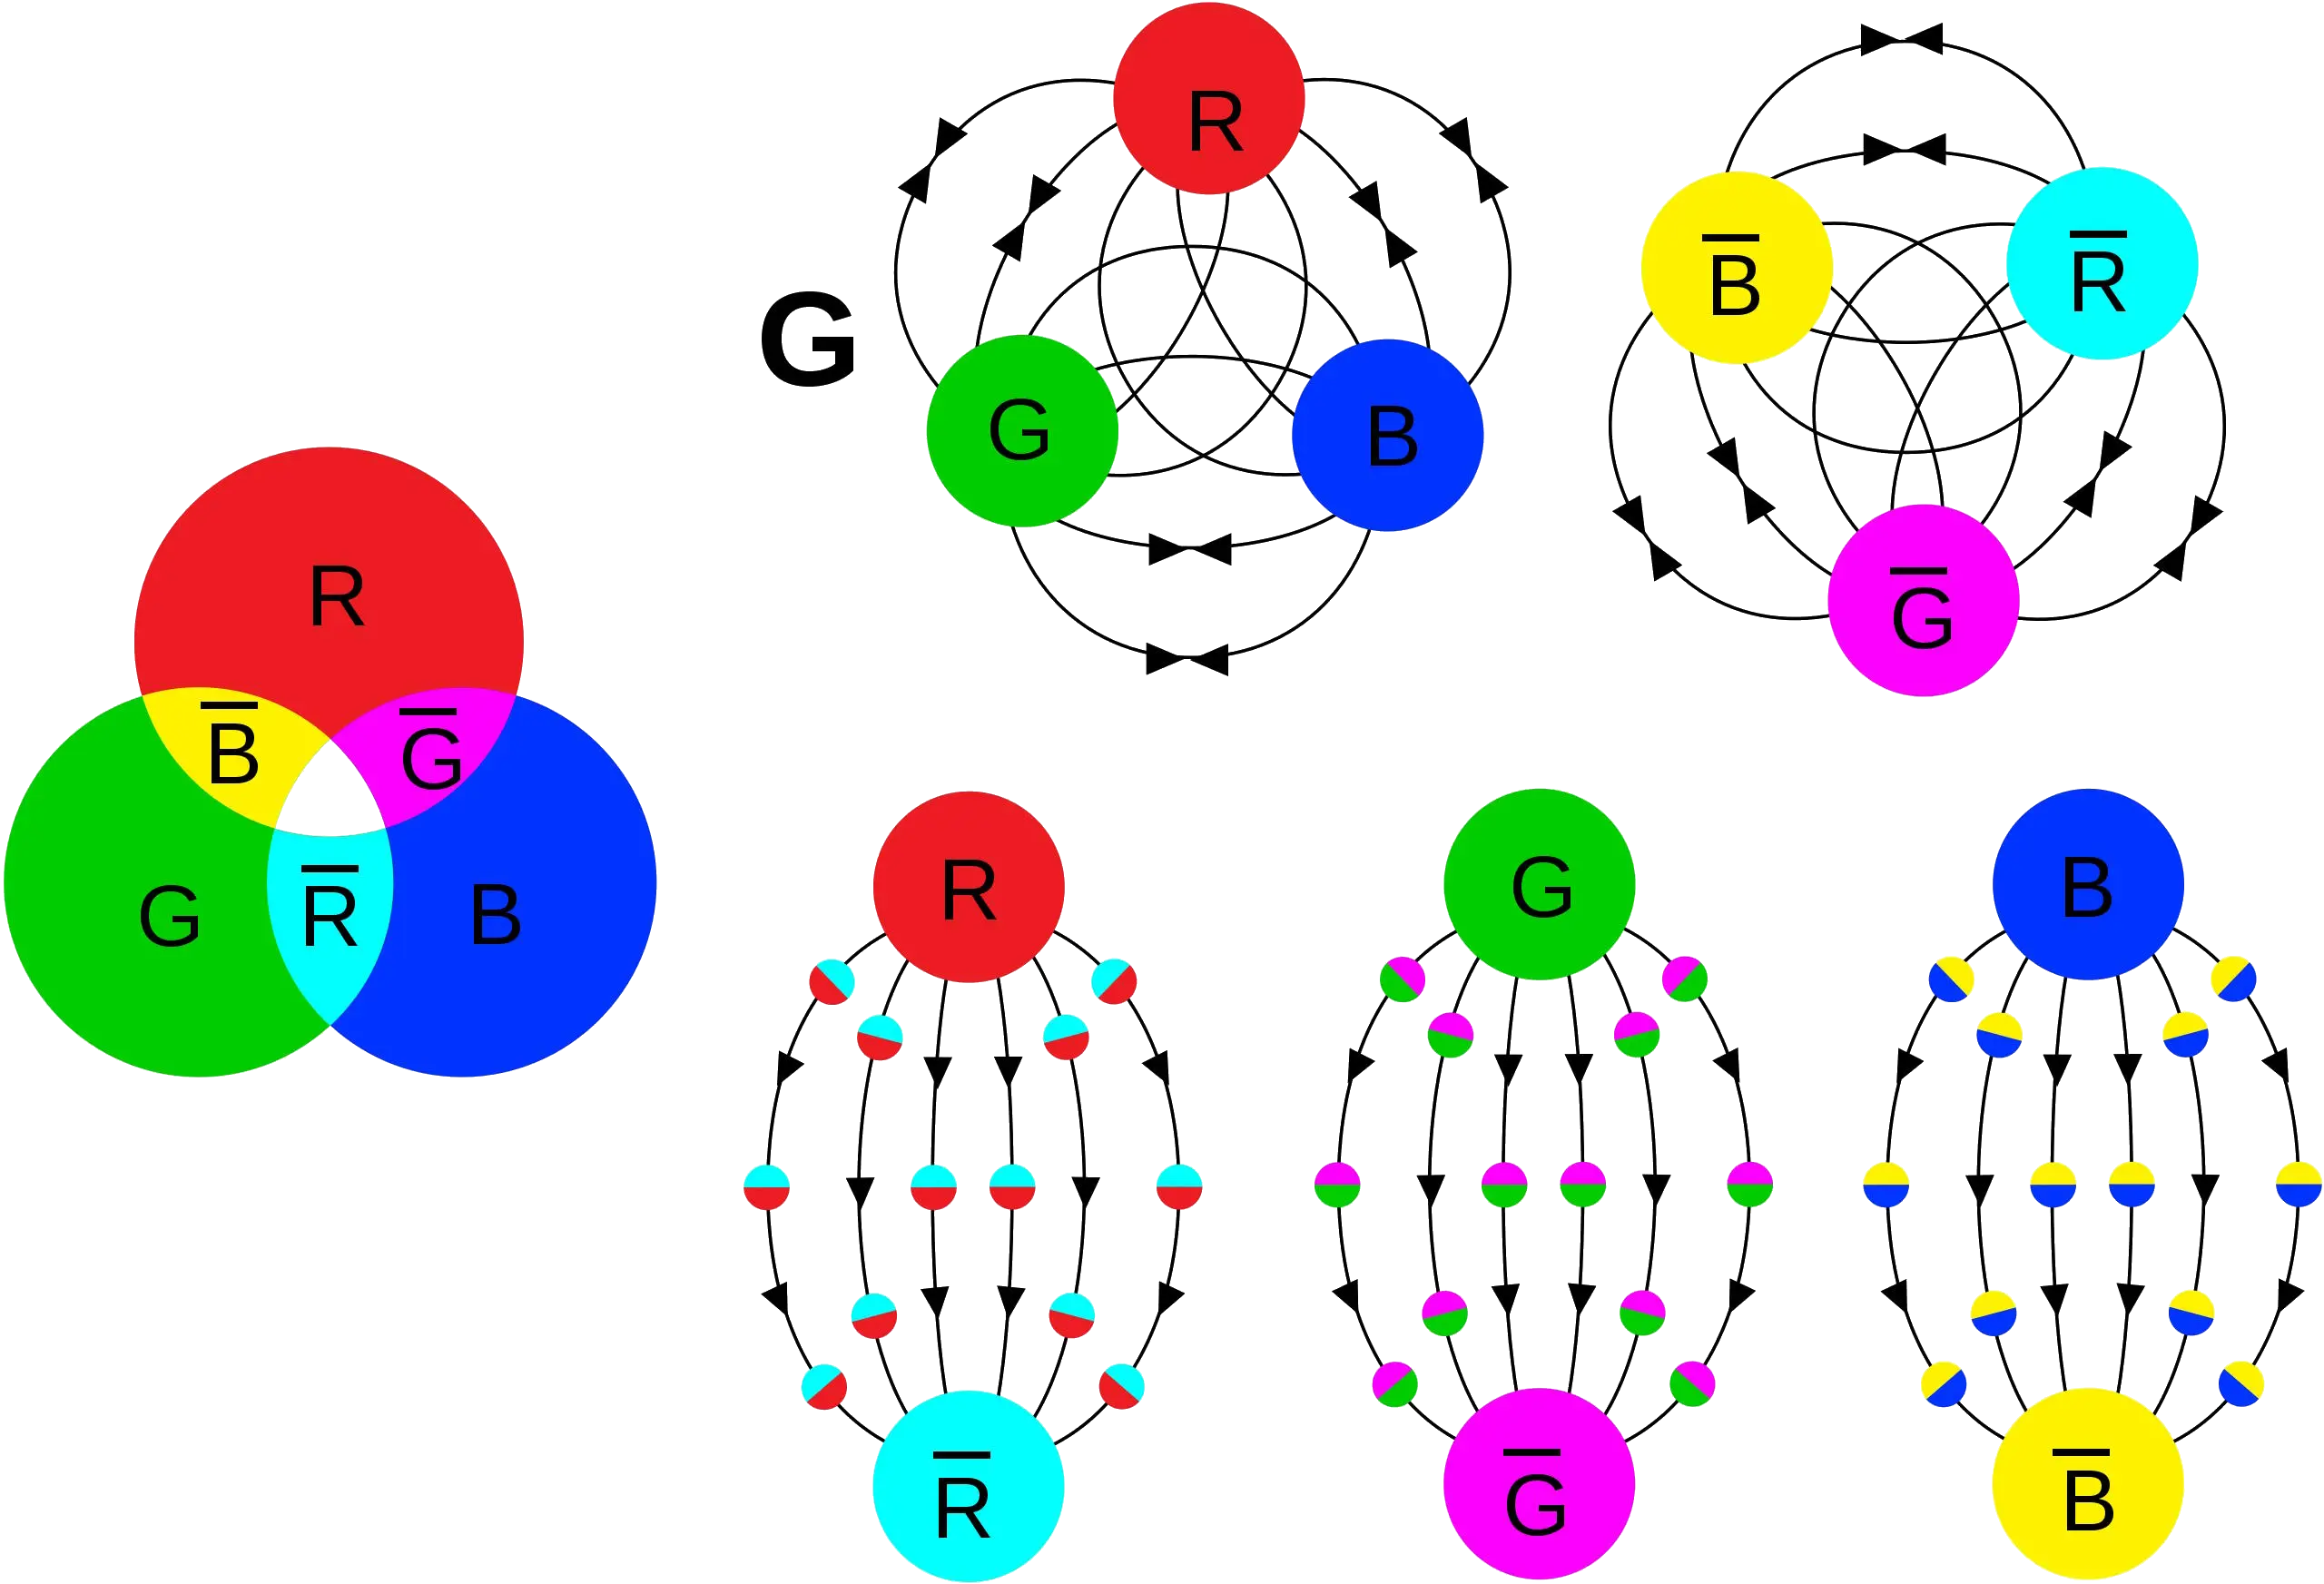
\includegraphics[width=\linewidth]{figures/gluon_cartoon.png} % opcional si tienes imagen de gluones
    }

  \end{columns}
\end{frame}

\begin{frame}{La presión total — Gas de Fermi ultrarrelativista}
  \begin{columns}
    \column{0.6\textwidth}

    \only<1>{
      \begin{equation*}
        \Xi^{\mathrm{FD}}(T, V, \mu) = \prod_{k=1}^\infty \left(1 + \xi e^{-\beta \varepsilon_k} \right)
      \end{equation*}
      \begin{equation*}
        \beta = \frac{1}{k_B T}, \quad \xi = e^{\beta \mu}
      \end{equation*}
    }

    \only<2>{
      \begin{align*}
        \Xi(T, V, \mu_+, \mu_-) &= \prod_{\varepsilon_+} \left(1 + \xi_+ e^{-\beta \varepsilon_+} \right)\\[0.5em]
        &\quad \times \prod_{\varepsilon_-} \left(1 + \xi_- e^{-\beta \varepsilon_-} \right)
      \end{align*}
      \vspace{0.5em}
      \begin{equation*}
        \xi_\pm = e^{\beta \mu_\pm}
      \end{equation*}
    }

    \only<3>{
      \begin{equation*}
        \langle n_k \rangle = \frac{1}{\xi^{-1} e^{\beta \varepsilon_k} + 1}
      \end{equation*}
      \vspace{-1em}
      \begin{align*}
        N_+ &= \sum_{\varepsilon_+} \langle n_+ \rangle = \sum_{\varepsilon_+} \frac{1}{\xi_+^{-1} e^{\beta \varepsilon_+} + 1} \\[0.5em]
        N_- &= \sum_{\varepsilon_-} \langle n_- \rangle = \sum_{\varepsilon_-} \frac{1}{\xi_-^{-1} e^{\beta \varepsilon_-} + 1}
      \end{align*}
    }

    \only<4>{
      \begin{equation*}
        q + \bar{q} \leftrightarrow \text{productos} + \Delta E
      \end{equation*}
      \begin{align*}
        dN_+ = dN_-, \quad &\Rightarrow \quad \mu_+ + \mu_- = 0 \quad \Rightarrow \quad \xi_+ \xi_- = 1 \\[0.5em]
        N &= N_+ - N_- = \sum_{\varepsilon > 0} \langle n_\varepsilon \rangle - \sum_{\varepsilon < 0} \langle n_\varepsilon \rangle
      \end{align*}
    }

    \only<5>{
      \begin{equation*}
        \langle n_\varepsilon \rangle = \frac{1}{e^{\beta (\varepsilon - \mu)} + 1}
      \end{equation*}
      \vspace{-0.5em}
      \begin{align*}
        N_+ &= \sum_{\varepsilon > 0} \langle n_\varepsilon \rangle \\[0.5em]
        N_- &= \sum_{\varepsilon < 0} \left(1 - \langle n_\varepsilon \rangle\right)
      \end{align*}
    }

    \column{0.4\textwidth}
    \centering
    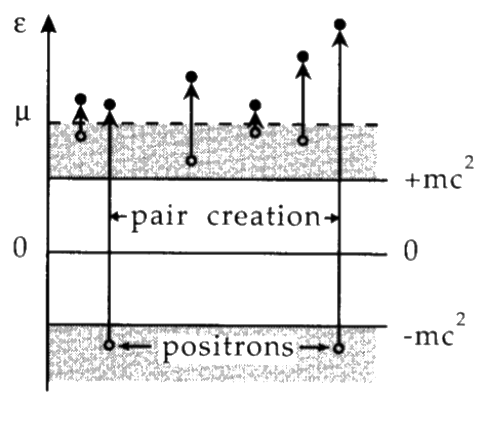
\includegraphics[width=\linewidth]{figures/creacion_pares.png}
  \end{columns}
\end{frame}

\begin{frame}{La presión total — Gas de Fermi ultrarrelativista 2}
  \begin{columns}
    % Columna izquierda: desarrollo animado de quarks
    \column{0.6\textwidth}

    % Animación paso a paso
    \only<1>{
      \begin{equation*}   
        N = N_+ - N_- = \sum_{\varepsilon_+} \frac{1}{e^{\beta(\varepsilon_+ - \mu)} + 1}
      \end{equation*}
      \begin{equation*}   
        - \sum_{\varepsilon_-} \frac{1}{e^{\beta(\varepsilon_- + \mu)} + 1}
      \end{equation*}
      \vspace{-0.3em}
      \begin{equation*}
        \Rightarrow \quad \frac{4\pi V}{(hc)^3} \int_0^\infty \varepsilon^2 d\varepsilon
        \left[ \frac{1}{e^{\beta(\varepsilon - \mu)} + 1} - \frac{1}{e^{\beta(\varepsilon + \mu)} + 1} \right]
      \end{equation*}
    }

    \only<2>{
      \textbf{Para quarks:}
      \begin{equation*}
        g_Q = N_s N_c N_f = 2 \times 3 \times 2 = 12
      \end{equation*}
      \begin{equation*}
        N_Q(T, V, \mu) = 4 g_Q \pi V \left( \frac{k_B T}{hc} \right)^3
      \end{equation*}
      \begin{equation*}
        \times \left[ \frac{\pi^2}{3} \left( \frac{\mu}{k_B T} \right)
        + \frac{1}{3} \left( \frac{\mu}{k_B T} \right)^3 \right]
      \end{equation*}
    }

    \only<3>{
      \begin{equation*}
        \hbar = k_B = c = 1
        \quad \Rightarrow \quad
      \end{equation*}
      \begin{equation*}
        N_Q = \frac{g_Q}{6} \left[ \frac{\mu}{T}
        + \frac{1}{\pi^2} \left( \frac{\mu}{T} \right)^3 \right] VT^3
      \end{equation*}
    }

    \only<4>{
      \begin{equation*}
        E = E_+ + E_- = \sum_{\varepsilon_+} \langle n_+ \rangle \varepsilon_+
        + \sum_{\varepsilon_-} \langle n_- \rangle \varepsilon_-
      \end{equation*}
      \begin{equation*}
        \Rightarrow \quad
        \frac{4\pi V}{(hc)^3} \int_0^\infty \varepsilon^3 d\varepsilon
        \left[ \frac{1}{e^{\beta(\varepsilon - \mu)} + 1}
        + \frac{1}{e^{\beta(\varepsilon + \mu)} + 1} \right]
      \end{equation*}
    }

    \only<5>{
      \begin{equation*}
        E_Q = g_Q \frac{4\pi V}{(hc)^3} (k_B T)^4
      \end{equation*}
      \begin{equation*}
        \times \left[ \frac{7 \pi^4}{60} + \frac{\pi^2}{2} \left( \frac{\mu}{k_B T} \right)^2
        + \frac{1}{4} \left( \frac{\mu}{k_B T} \right)^4 \right]
      \end{equation*}
    }

    \only<6>{
      \begin{equation*}
        \hbar = k_B = c = 1 \quad \Rightarrow \quad
      \end{equation*}
      \begin{equation*}
        E_Q = g_Q \left[ \frac{7 \pi^2}{120}
        + \frac{1}{4} \left( \frac{\mu}{T} \right)^2
        + \frac{1}{8\pi^2} \left( \frac{\mu}{T} \right)^4 \right] VT^4
      \end{equation*}
    }

    % Columna derecha: imagen fija (quarks caricaturizados)
    \column{0.4\textwidth}
    \centering
    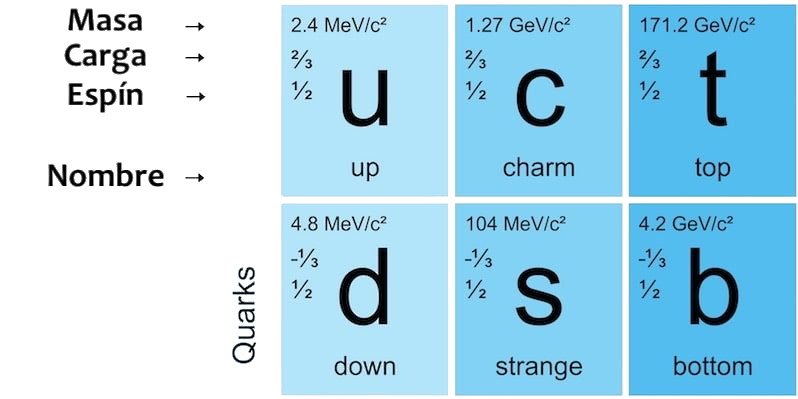
\includegraphics[width=\linewidth]{figures/quark_cartoon.png}
  \end{columns}
\end{frame}

\begin{frame}{Presión total dentro del hadrón}
  \begin{columns}
    \column{0.6\textwidth}
    \textbf{Contribuciones individuales:}
    \begin{align*}
      P_G &= g_G \frac{\pi^2}{90} T^4 \\
      P_Q &= \frac{g_Q}{6} \left[ \frac{7\pi^2}{60}
      + \frac{1}{2} \left( \frac{\mu}{T} \right)^2
      + \frac{1}{2\pi^2} \left( \frac{\mu}{T} \right)^4 \right] T^4
    \end{align*}

    \vspace{1em}
    \textbf{Presión total:}
    \begin{equation*}
      P_{\text{total}} = P_G + P_Q
    \end{equation*}

    \column{0.4\textwidth}
    \centering
    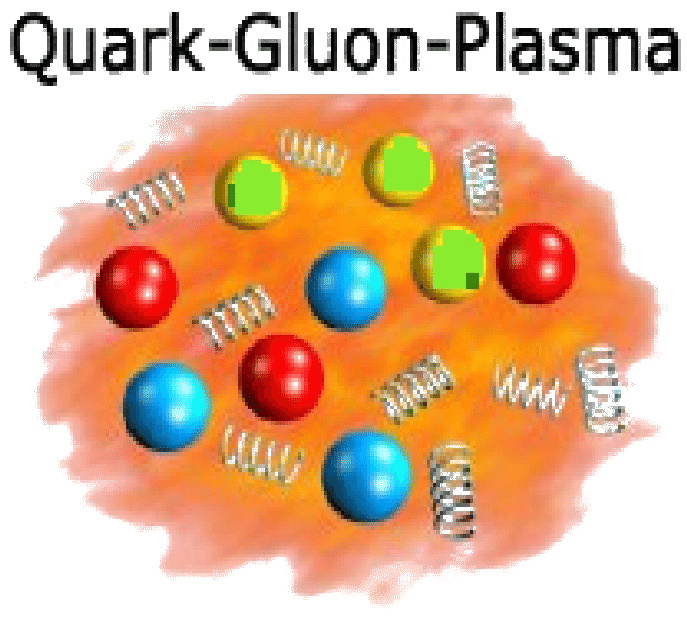
\includegraphics[width=\linewidth]{figures/QG-plasma.png}
  \end{columns}
\end{frame}
%%%%%%%%%%%%%%%%%%%%%%%%%%%%%%%%%%%%%%%%%%%%%%%%%%%%%%%%%%%%%%%%%%%%%%%%%%%%%%%%%%%%%

\section[Extensión con Estadística de Tsallis]{3. Extensión con Estadística de Tsallis}
\begin{frame}{La estadística de Tsallis}
  \begin{columns}
    \column{0.4\textwidth}
    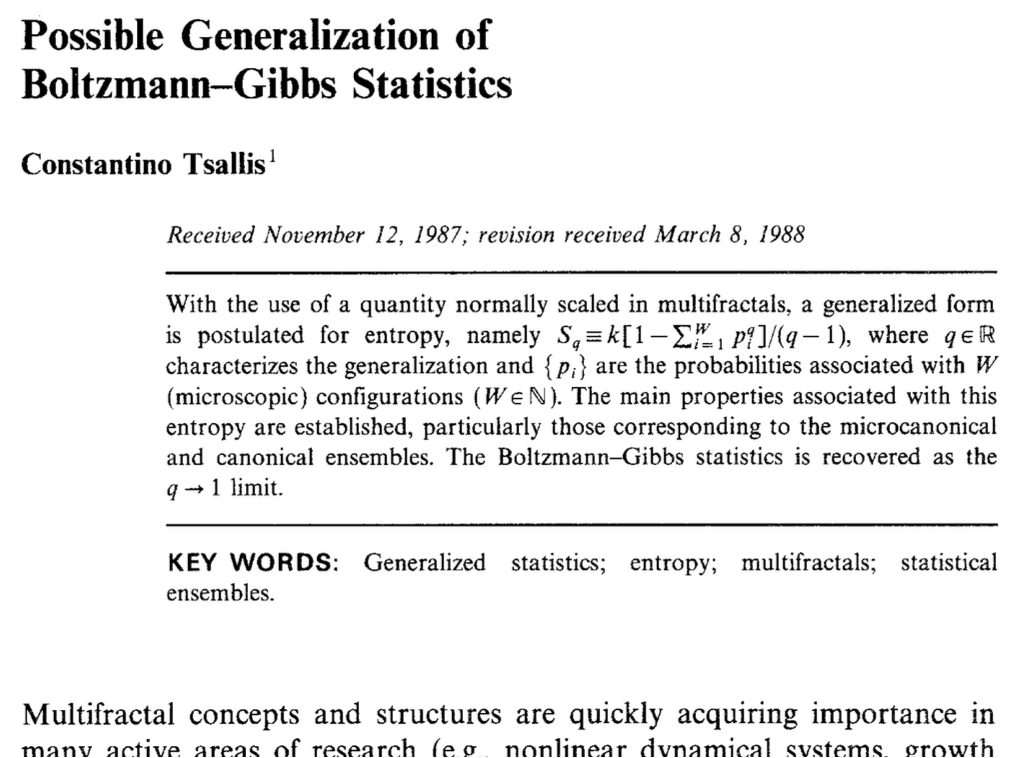
\includegraphics[width=\linewidth]{figures/tsallis_1988.png} % artículo original escaneado

    \column{0.6\textwidth}

    \only<1>{
      \begin{equation*}
        S_q \equiv k_{\text{B}} \frac{1 - \sum_{i=1}^{W} p_i^q}{q - 1} \quad (q \in \mathbb{R})
      \end{equation*}
    }

    \only<2>{
      \begin{equation*}
        S_q \equiv k_{\text{B}} \frac{1 - \sum_{i=1}^{W} p_i^q}{q - 1}
      \end{equation*}
      \vspace{-1em}
      \begin{equation*}
        S_1 \equiv \lim_{q \to 1} S_q = k_{\text{B}} \lim_{q \to 1} \frac{1 - \sum_{i=1}^{W} p_i^q}{q - 1}
      \end{equation*}
      \begin{equation*}
        = -k_{\text{B}} \sum_{i=1}^{W} p_i \ln p_i
      \end{equation*}
    }

    \only<3>{
      \begin{equation*}
        S_q = k_{\text{B}} \frac{1 - \sum_{i=1}^{W} p_i^q}{q - 1}
      \end{equation*}
      \vspace{-1em}
      \begin{equation*}
        S_1 = -k_{\text{B}} \sum_{i=1}^{W} p_i \ln p_i
      \end{equation*}
      \vspace{-1em}
      \begin{block}{Aditividad (independencia estadística)}
        \[
        \sum_{i,j}^{W_A,W_B} (p_{ij}^{A \cup B})^q = 
        \left[ \sum_{i=1}^{W_A} (p_i^A)^q \right] \left[ \sum_{j=1}^{W_B} (p_j^B)^q \right]
        \]
        \[
        \frac{S_q(A + B)}{k_{\text{B}}} = \frac{S_q(A)}{k_{\text{B}}} + \frac{S_q(B)}{k_{\text{B}}}
        \]
        \[
        \quad  + (1 - q) \frac{S_q(A)}{k_{\text{B}}} \frac{S_q(B)}{k_{\text{B}}}
        \]
      \end{block}
    }
  \end{columns}
\end{frame}

\begin{frame}{¿Por qué la estadística de Tsallis?}
  \framesubtitle{Justificación fenomenológica: turbulencia, rayos cósmicos y física de altas energías}

  \begin{columns}
    % COLUMNA IZQUIERDA: cambia contenido según paso
    \column{0.45\textwidth}

    \only<1>{
      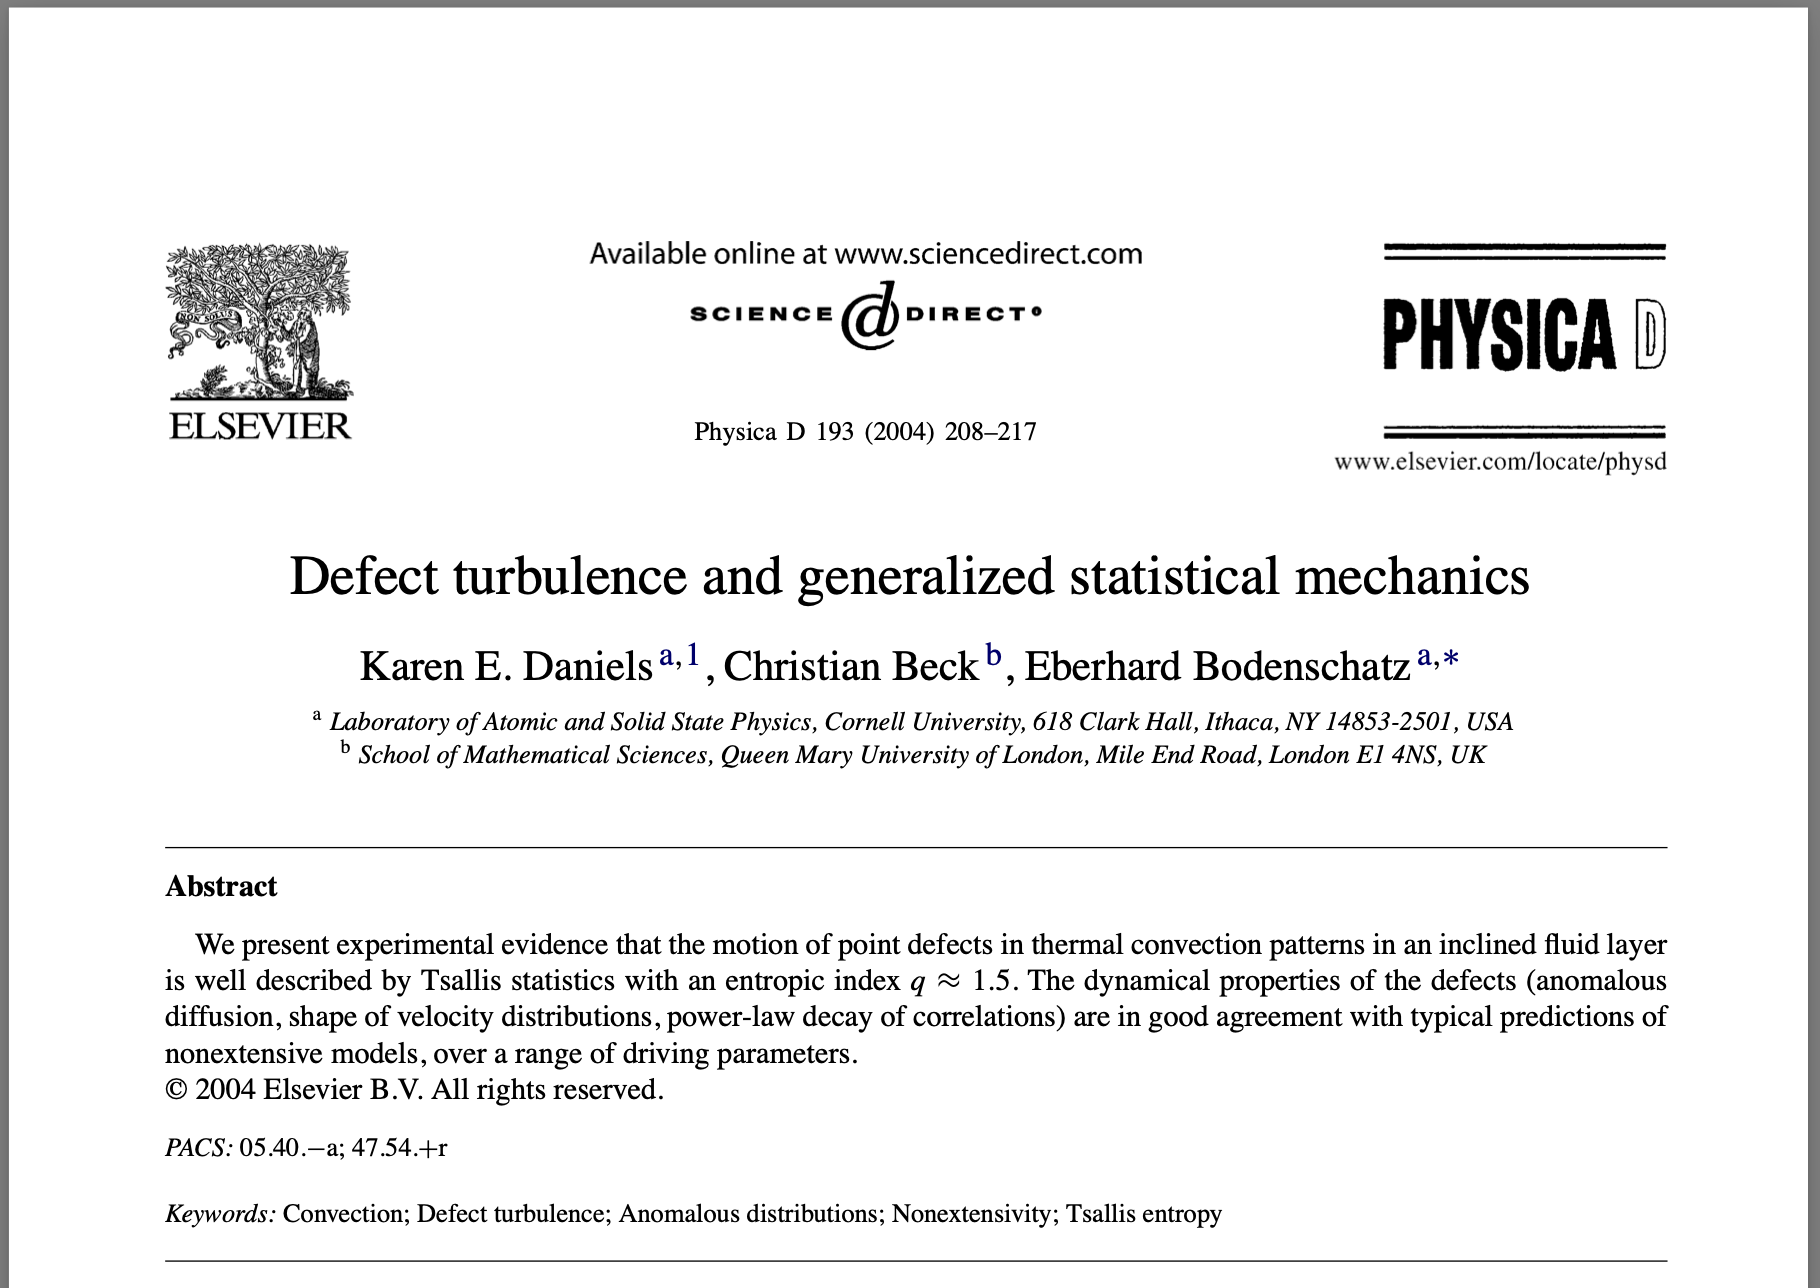
\includegraphics[width=\linewidth]{figures/daniels_2004_turbulence.png}
    }

    \only<2>{
      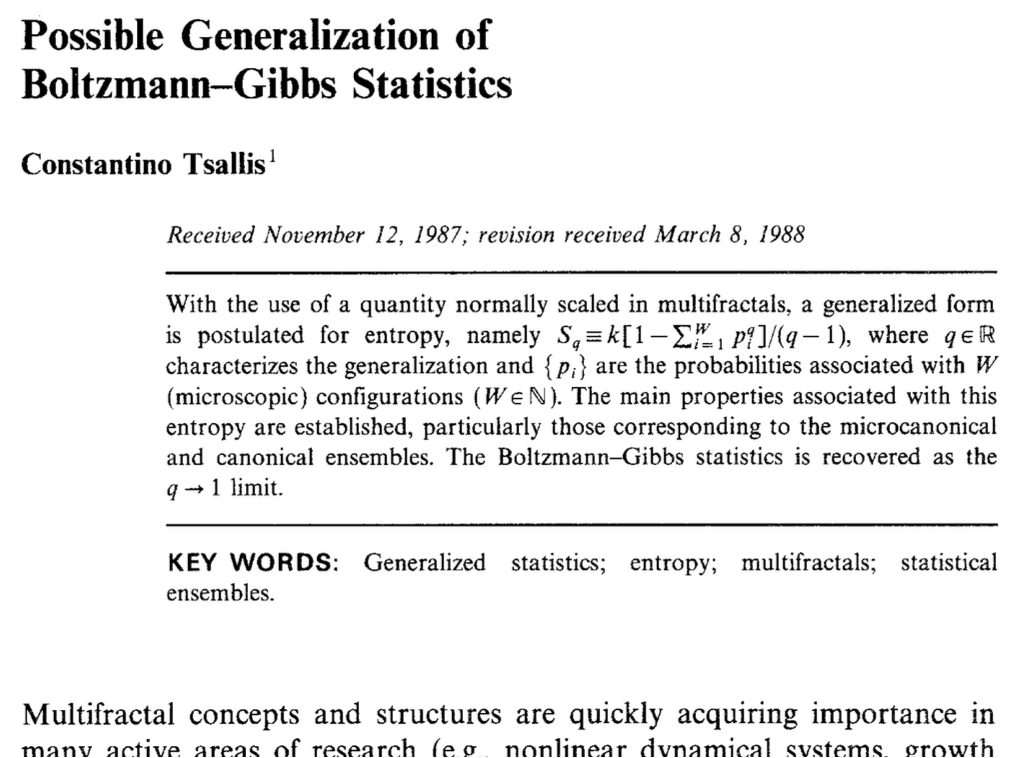
\includegraphics[width=\linewidth]{figures/tsallis_1988.png}
    }

    % COLUMNA DERECHA: cambia contenido según paso
    \column{0.55\textwidth}

    \only<1>{
      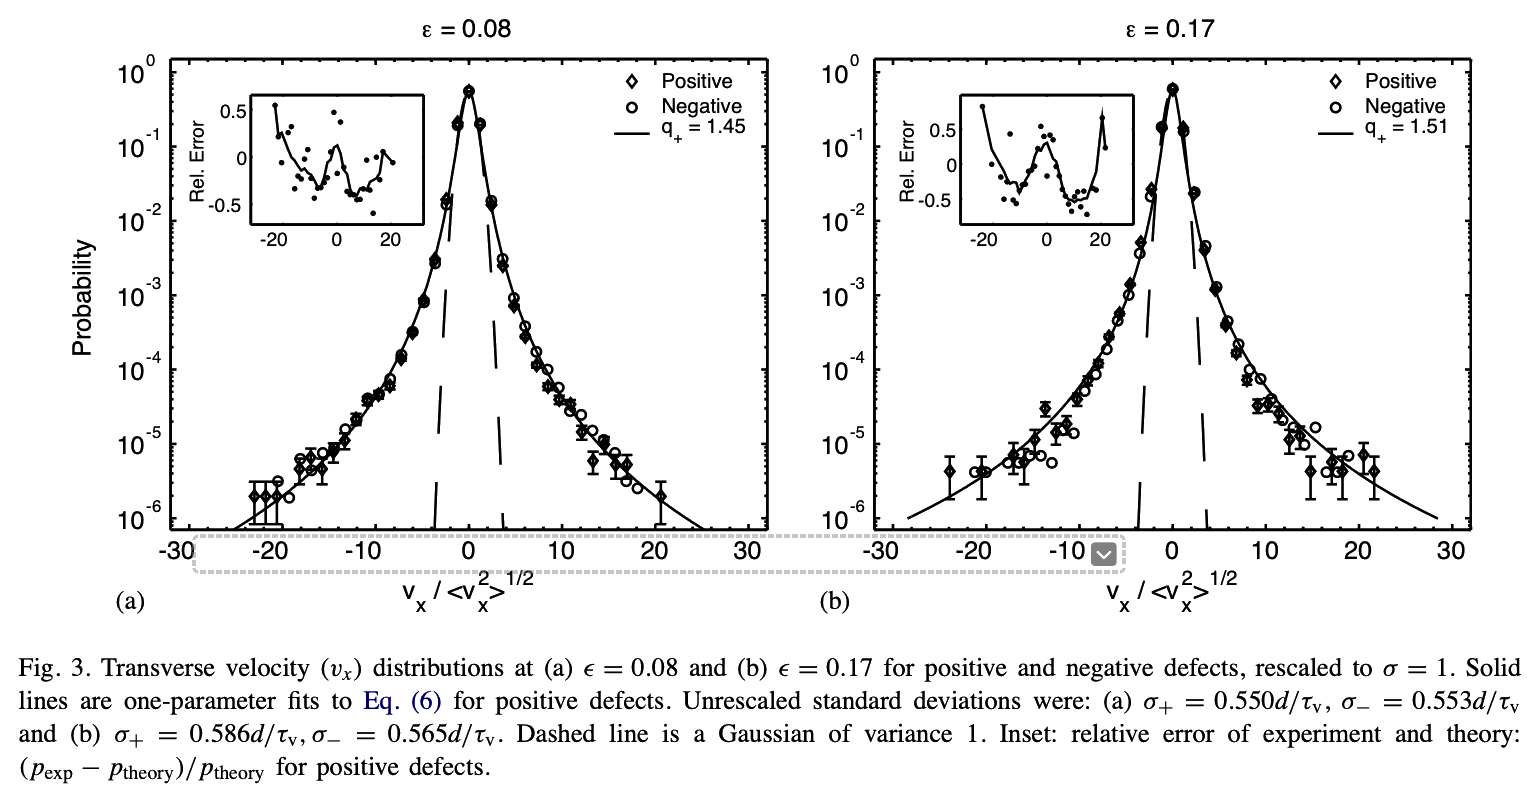
\includegraphics[width=\linewidth]{figures/defect_turbulence_fits.png}
    }

    \only<2>{
      \begin{columns}
        \column{0.48\textwidth}
        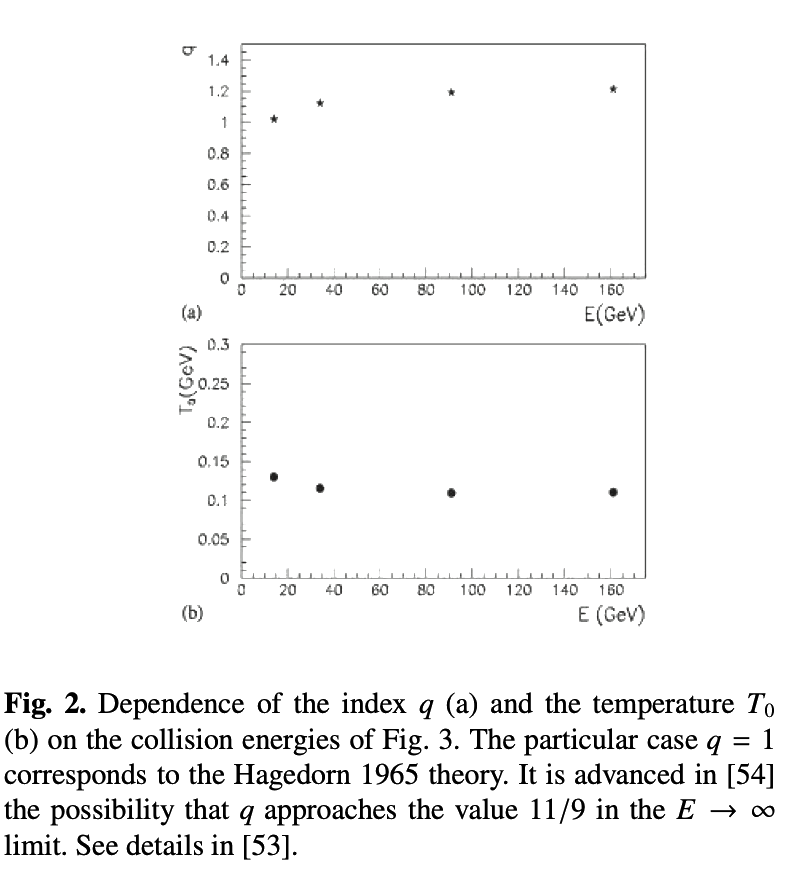
\includegraphics[width=\linewidth]{figures/q_vs_energy.png}

        \column{0.48\textwidth}
        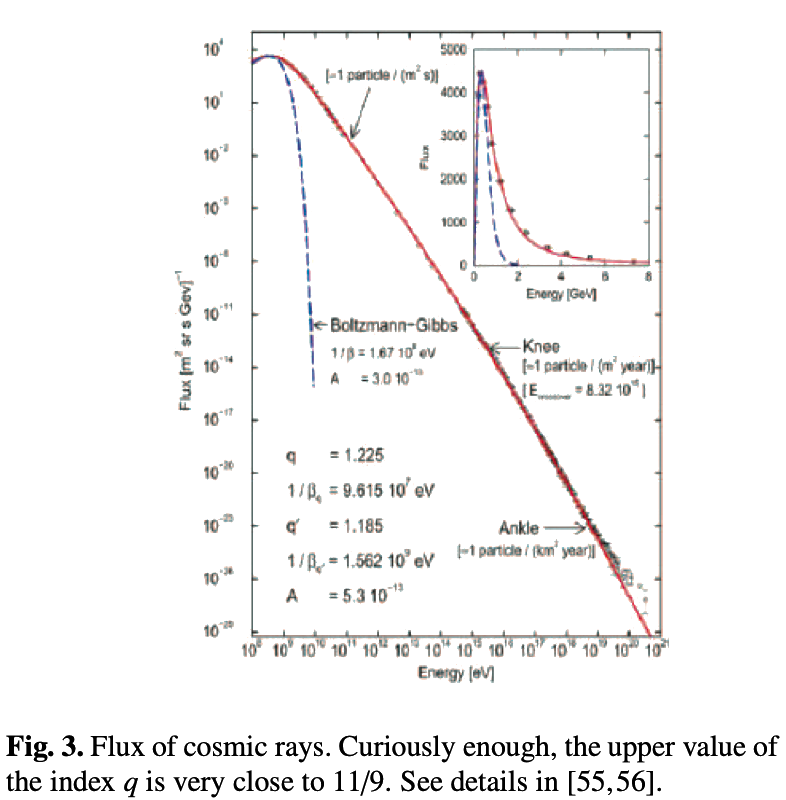
\includegraphics[width=\linewidth]{figures/cosmic_rays_fit.png}
      \end{columns}
    }

  \end{columns}
\end{frame}


\begin{frame}{Tsallis MIT bag model}
  \begin{itemize}
    \only<1>{
      \item En el trabajo en desarrollo proponemos una descripción fenomenológica basada en el modelo de bolsa del MIT y una aproximación no extensiva estadística referida como modelo de bolsa \textbf{T-MIT} para abreviar \textit{Tsallis MIT Bag Model}\textsuperscript{2}.
    }
    \only<2>{
      \item En el trabajo en desarrollo proponemos una descripción fenomenológica basada en el modelo de bolsa del MIT y una aproximación no extensiva estadística referida como modelo de bolsa \textbf{T-MIT} para abreviar \textit{Tsallis MIT Bag Model}\textsuperscript{2}.
      \item En el modelo de bolsa de T-MIT uno puede estimar no solo la distribución de presión total sino también esa debida a los gluones dentro del protón.
    }
    \only<3>{
      \item En el trabajo en desarrollo proponemos una descripción fenomenológica basada en el modelo de bolsa del MIT y una aproximación no extensiva estadística referida como modelo de bolsa \textbf{T-MIT} para abreviar \textit{Tsallis MIT Bag Model}\textsuperscript{2}.
      \item En el modelo de bolsa de T-MIT uno puede estimar no solo la distribución de presión total sino también esa debida a los gluones dentro del protón.
      \item Sin embargo, para ello hacemos uso de la distribución de presión de quarks publicada en \textit{Nature, Vol. 557, No. 7705}.
    }
  \end{itemize}

  \vspace{1em}
  {\tiny\textsuperscript{2}Este modelo integra diferentes aspectos de materia hadrónica permitiendo estudiar en más detalle procesos donde un potencial distinto de cero entra.}
\end{frame}

%%%%%%%%%%%%%%%%%%%%%%%%%%%%%%%%%%%%%%%%%%%%%%%%%%%%%%%%%%%%%%%%%%%%%%%%%%%%%%%%%%%%%

\section[La presión dentro del hadrón]{4. La presión dentro del hadrón}





%%%%%%%%%%%%%%%%%%%%%%%%%%%%%%%%%%%%%%%%%%%%%%%%%%%%%%%%%%%%%%%%%%%%%%%%%%%%%%%%%%%%%
\section[Resultados]{5. Resultados}
\begin{frame}{Perfil de presión radial}
  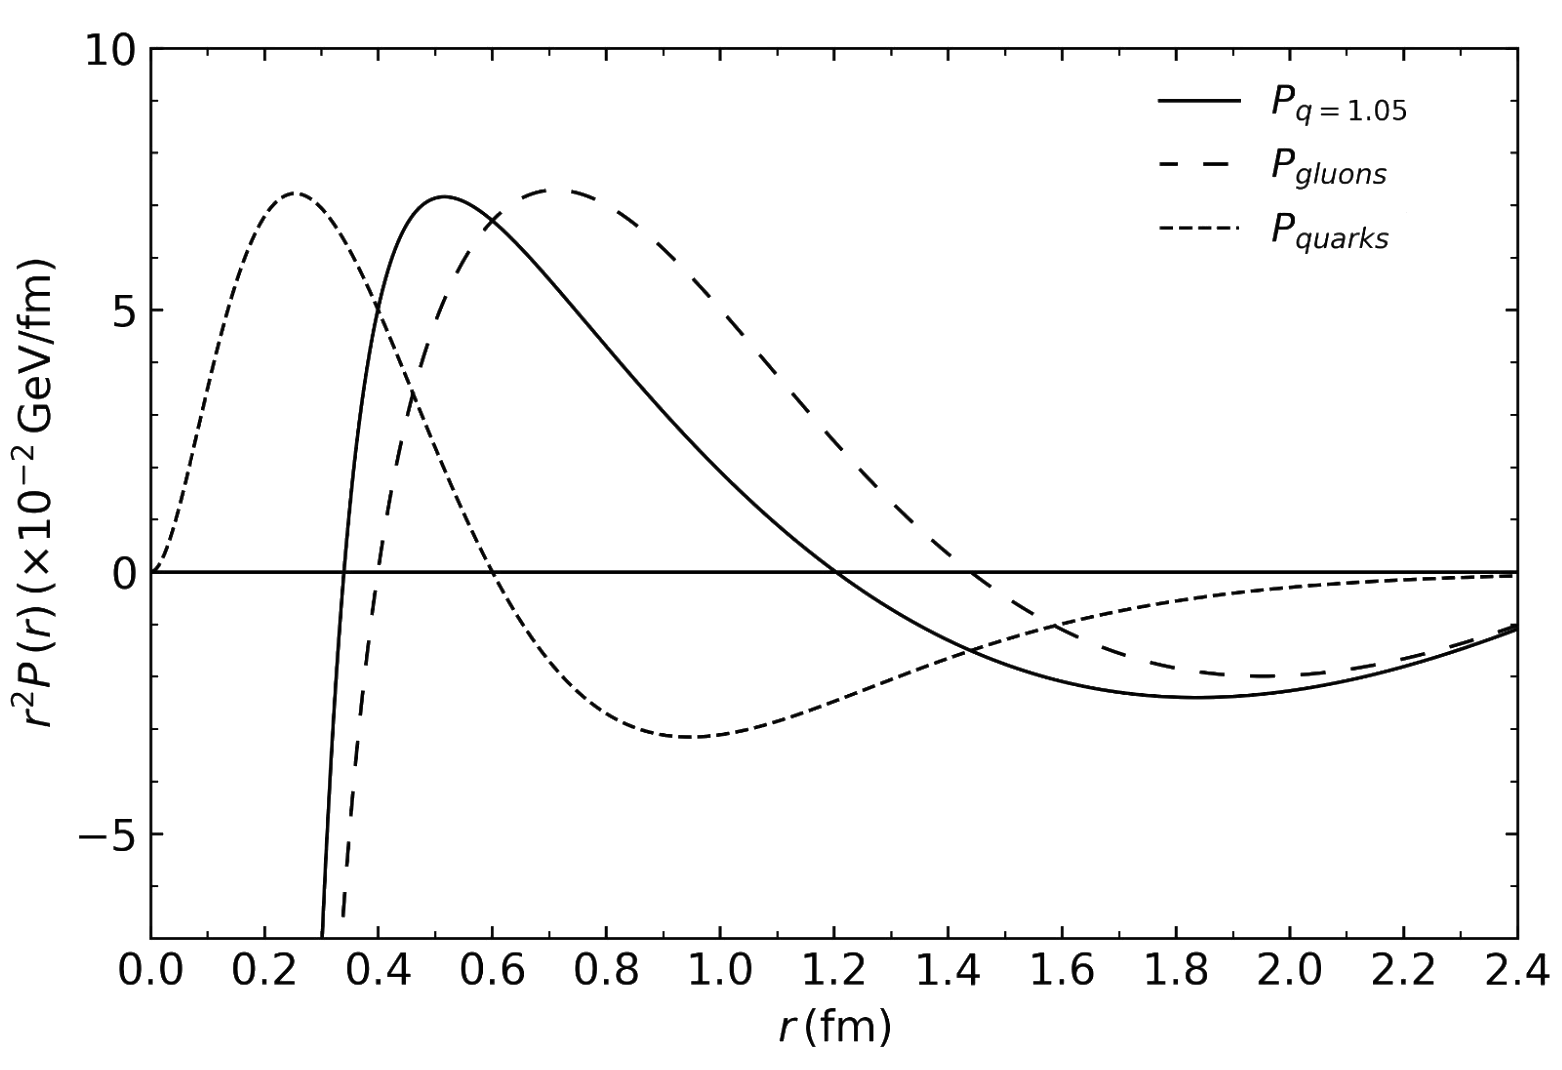
\includegraphics[width=0.8\textwidth]{figures/PressureDistributionsTot-Q-G.png}
  \begin{itemize}
    \item Comparación con resultados de LQCD
    \item Coincidencia con \( r^2 P(r) \) en DVCS
  \end{itemize}
\end{frame}

\begin{frame}{Descomposición de presión}
  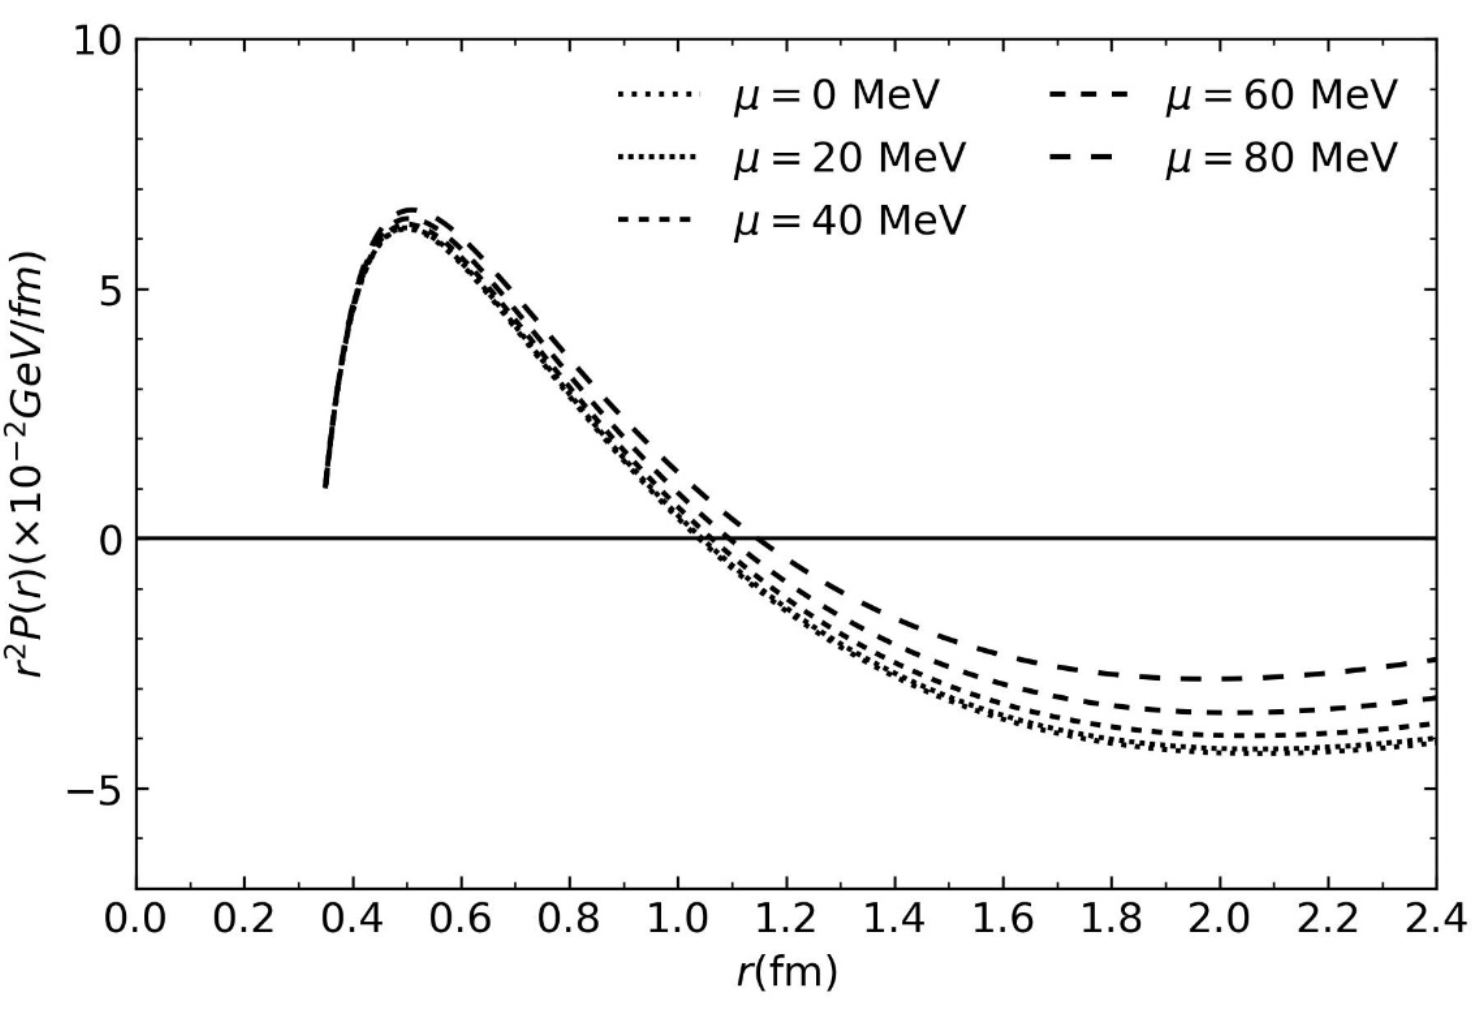
\includegraphics[width=0.7\textwidth]{TotalPressureTsallis.png}
  \begin{itemize}
    \item Presión total \( P_q \)
    \item Presión gluónica \( P_G \)
  \end{itemize}
\end{frame}
%%%%%%%%%%%%%%%%%%%%%%%%%%%%%%%%%%%%%%%%%%%%%%%%%%%%%%%%%%%%%%%%%%%%%%%%%%%%%%%%%%%%%
\section[Interpretación del parámetro \( q \)]{6. Interpretación del parámetro \( q \)}
\begin{frame}{Relación \( q(r) \leftrightarrow B(r) \)}
  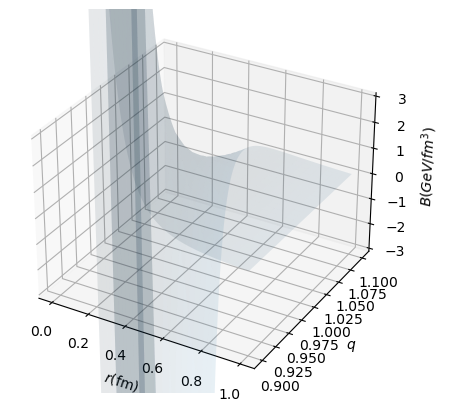
\includegraphics[width=0.7\textwidth]{B_vs_q_vs_r.png}
  \begin{itemize}
    \item Superficie reconstruida de \( B(q, r) \)
    \item Divergencias para \( q < 1 \), interpretables
  \end{itemize}
\end{frame}

\begin{frame}{Cortes radiales y visualización}
  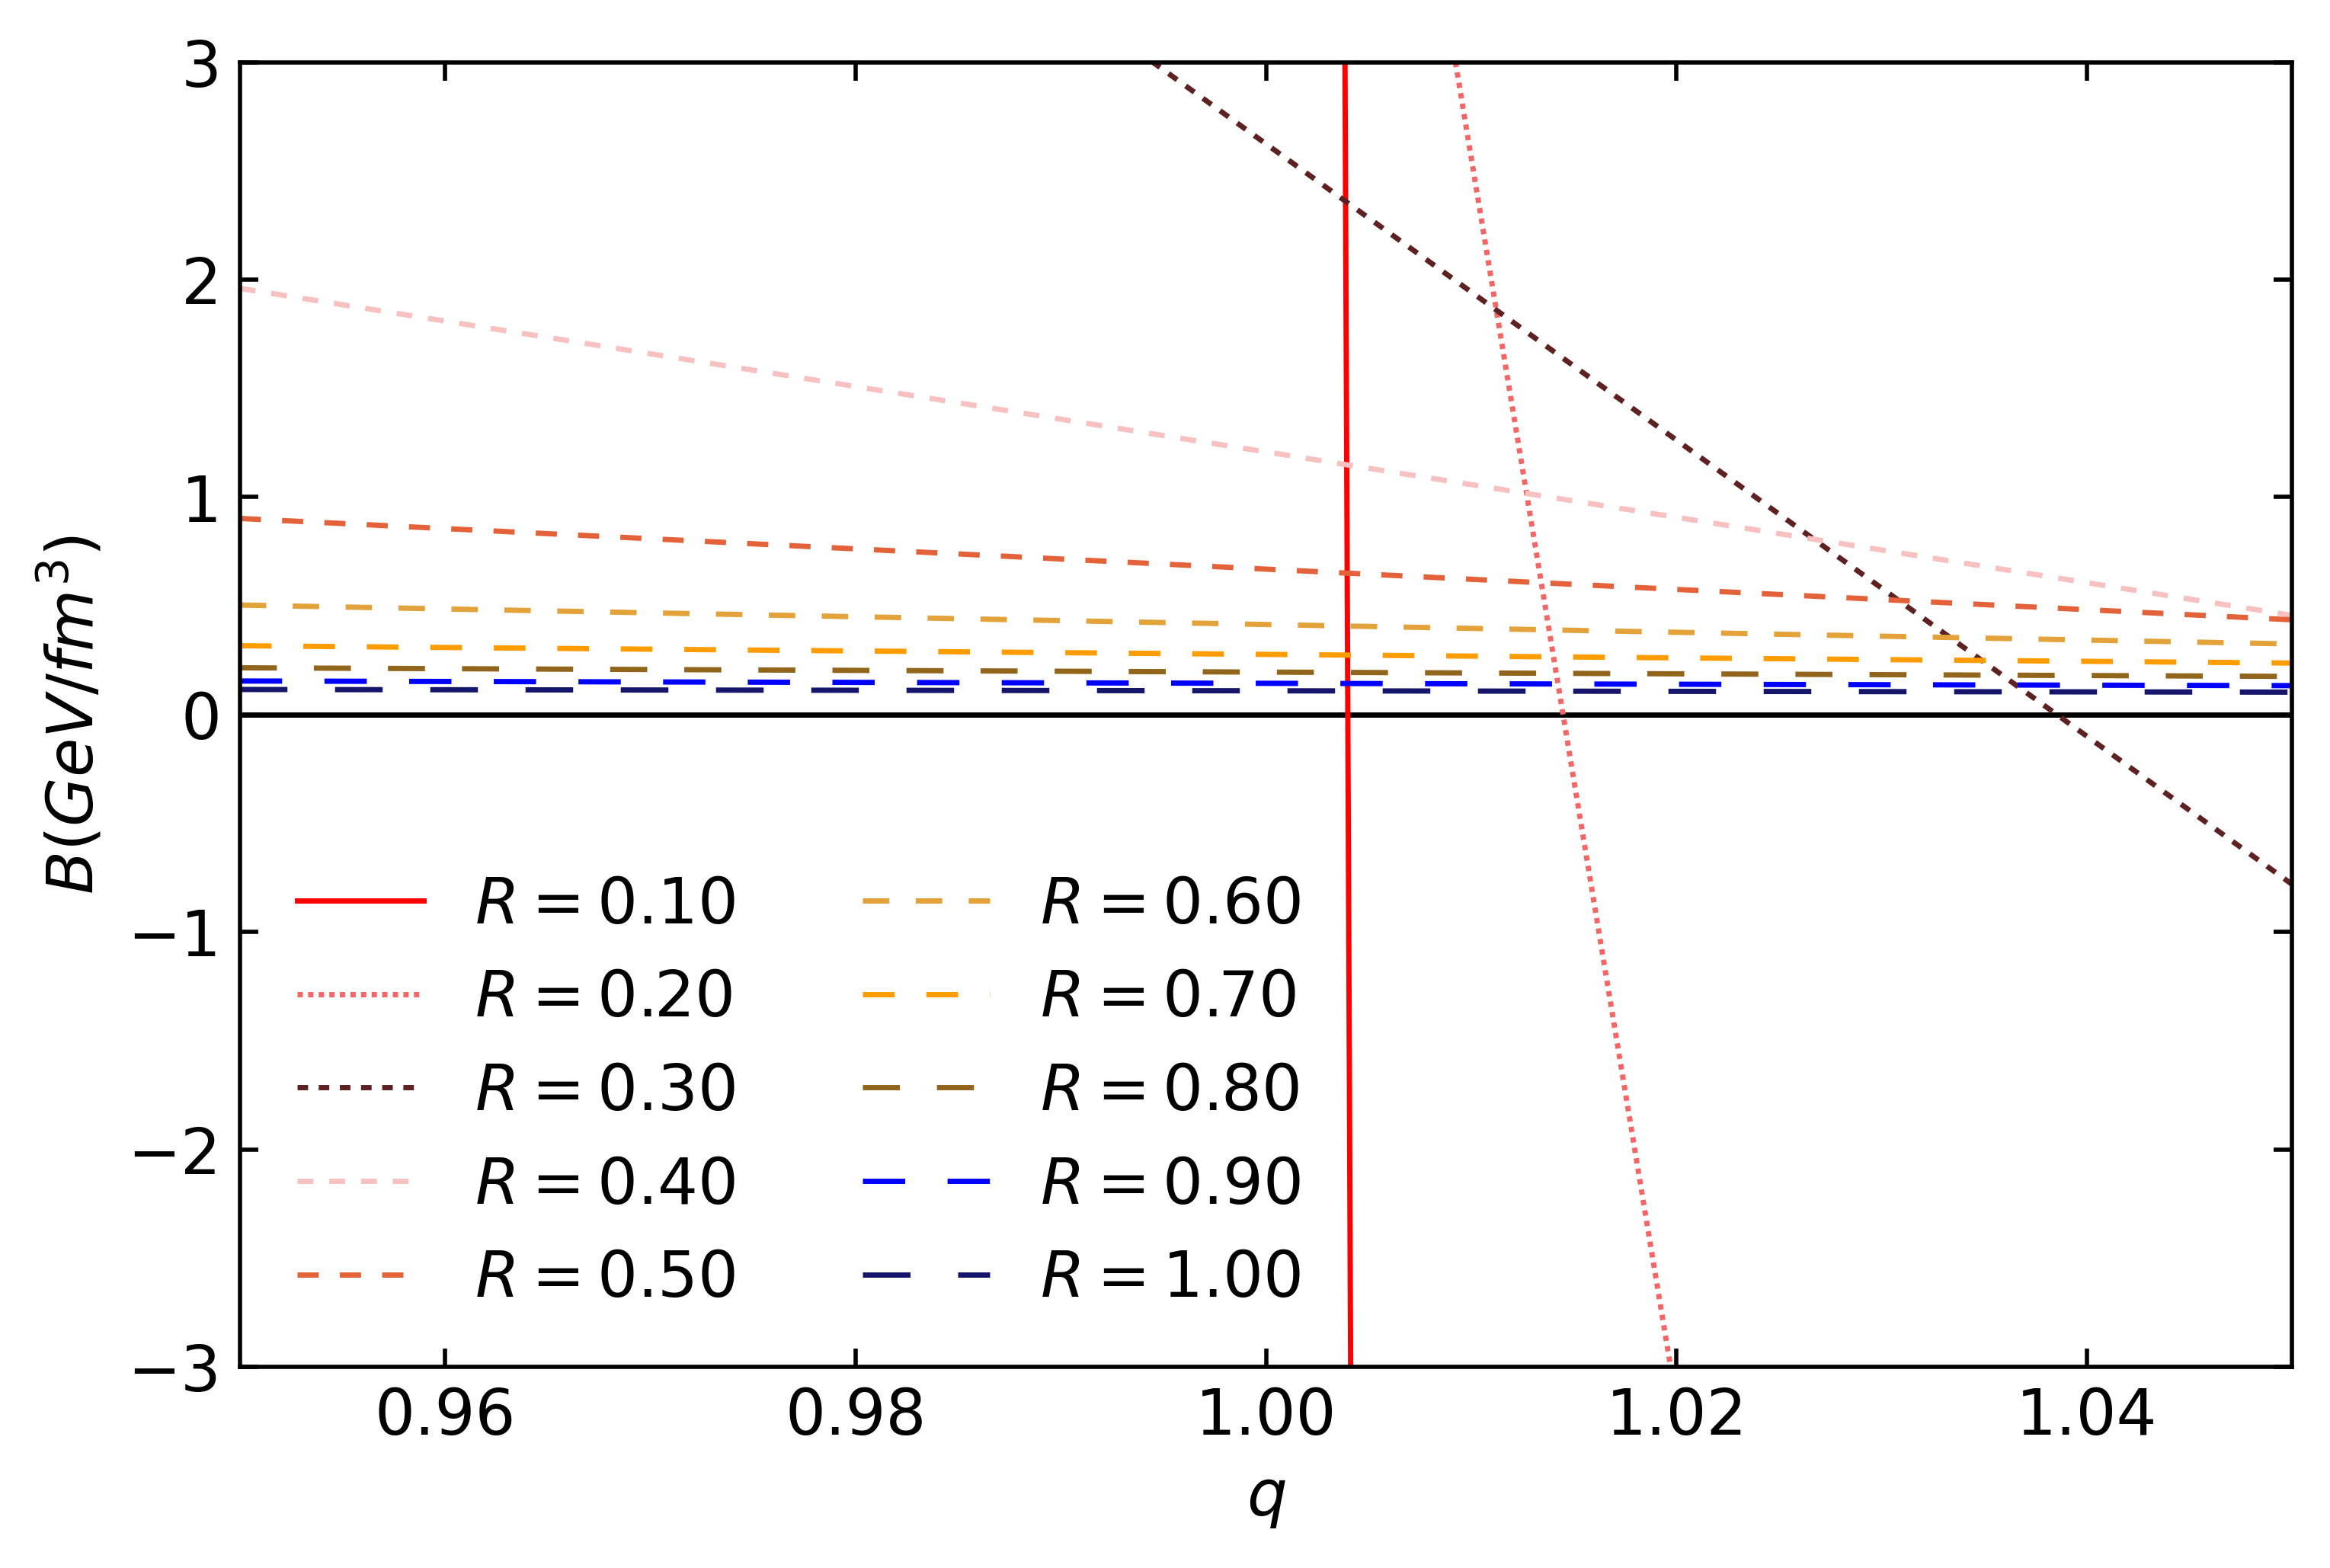
\includegraphics[width=0.75\textwidth]{BvsQcuts.png}
  \begin{itemize}
    \item Aproximación lineal entre \( q \) y \( B \) para \( r > 0.6\, \mathrm{fm} \)
  \end{itemize}
\end{frame}
%%%%%%%%%%%%%%%%%%%%%%%%%%%%%%%%%%%%%%%%%%%%%%%%%%%%%%%%%%%%%%%%%%%%%%%%%%%%%%%%%%%%%
\section[Exploraciones adicionales]{7. Exploraciones adicionales}
\begin{frame}{Reconstrucción de \( B(r) \)}
  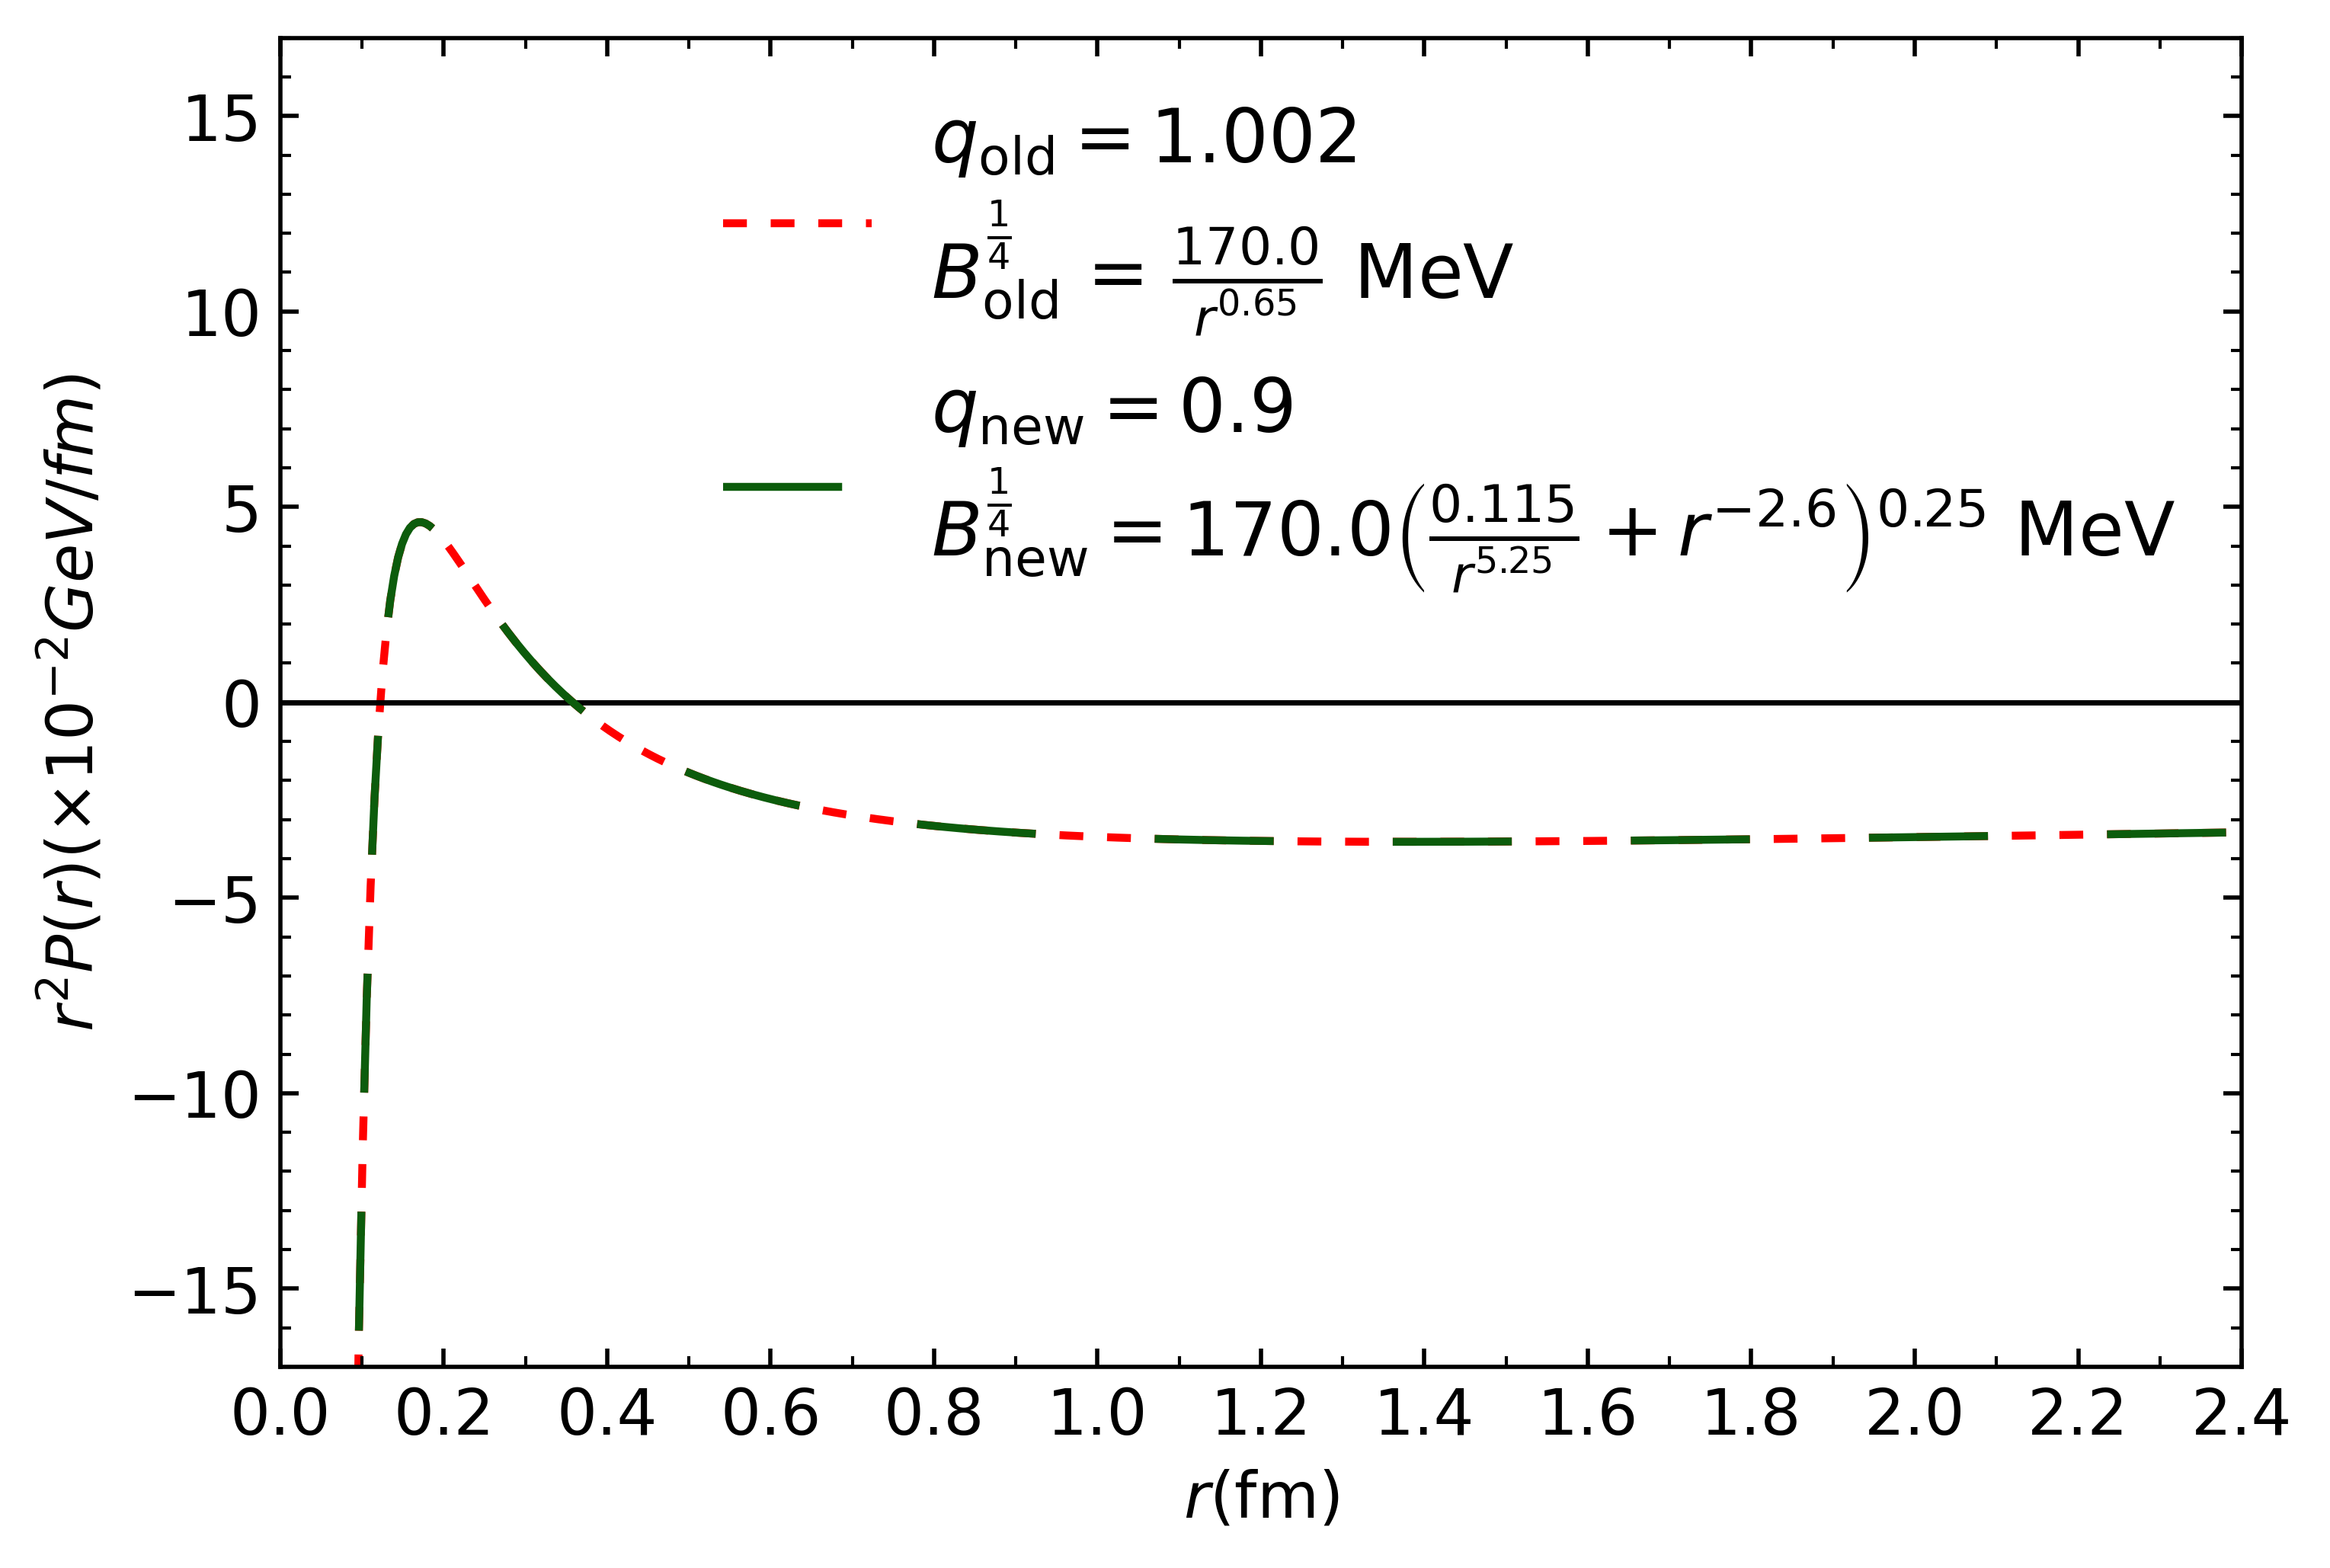
\includegraphics[width=0.75\textwidth]{Comparacion_B_old_new_combined.png}
  \begin{itemize}
    \item Dos configuraciones \( q = 1.002 \) y \( q = 0.9 \)
    \item Resultados consistentes en presión
  \end{itemize}
\end{frame}

\begin{frame}{¿Y si intentamos predecir \( q \)?}
  \begin{itemize}
    \item Intento de cálculo desde energía de Tsallis: limitado
    \item Propuesta: aprendizaje automático
    \item Futuro: entrenar con perfiles conocidos
  \end{itemize}
\end{frame}
%%%%%%%%%%%%%%%%%%%%%%%%%%%%%%%%%%%%%%%%%%%%%%%%%%%%%%%%%%%%%%%%%%%%%%%%%%%%%%%%%%%%%
\section[Conclusiones]{8. Conclusiones}
\begin{frame}{Resumen y perspectivas}
  \begin{itemize}
    \item \( q \) puede sustituir a \( B \) bajo ciertas condiciones
    \item Modelo accesible y reproducible computacionalmente
    \item Futuros trabajos: ML, ajuste directo, exploraciones hadrónicas
  \end{itemize}
\end{frame}

\begin{frame}[standout]
  \centering
  \Large ¡Gracias por su atención!
  \centering
  \Huge ¿Preguntas?
\end{frame}

% Bibliografía si aplica
\appendix
\begin{frame}[allowframebreaks]{Bibliografía}
  \printbibliography
\end{frame}


\end{document}